\subsection{Inverse systems of measures}

DEFINITION 1. --- Let \(\mathcal{T} = (\mathrm{T}_i, p_{ij})\) be an inverse system of topological spaces indexed by I. One calls inverse system (resp. sub-inverse system)

of measures on \(\mathcal{T}\) a family \((\mu_i)_{i\in I}\) , where \(\mu_i\) is a bounded measure on \(\mathrm{T}_i\) for all \(i\in \mathrm{I}\) , and where \(\mu_i = p_{ij}(\mu_j)\) (resp. \(\mu_i\geqslant p_{ij}(\mu_j)\) ) for \(i\leqslant j\) .

PROPOSITION 3. --- Let there be given an inverse system of topological spaces \(\mathcal{T} = (\mathrm{T}_i, p_{ij})\) indexed by I, a topological space T, a coherent and separating family of continuous mappings \(p_i: \mathrm{T} \to \mathrm{T}_i\) (for \(i \in \mathrm{I}\) ) and a sub-inverse system \((\mu_i)_{i \in \mathrm{I}}\) of measures on \(\mathcal{T}\) . For every compact subset K of T, set

\[
\mathrm{J} (\mathrm{K}) = \inf _ {i \in \mathrm{I}} \mu_ {i} ^ {\bullet} (p _ {i} (\mathrm{K})).\tag{1}
\]

Then there exists a bounded measure \(\pi\) on T, and only one, such that \(\pi^{\bullet}(\mathrm{K}) = \mathrm{J}(\mathrm{K})\) for every compact subset K of T. One has \(\mu_i \geqslant p_i(\pi)\) for all \(i \in I\) , and \(\pi\) is the largest measure on T satisfying this condition.

Let us first prove that \(\mathrm{J}(\mathrm{K})\) is the limit of \(\mu_i^\bullet (p_i(\mathrm{K}))\) with respect to the section filter \(\mathfrak{F}\) of the directed preordered set I: for this, it suffices (GT, IV, §5, No.~2, Th. 2) to show that \(\mu_i^\bullet (p_i(\mathrm{K})) \geqslant \mu_j^\bullet (p_j(\mathrm{K}))\) for \(i \leqslant j\) ; now, setting \(\mu_{ij}' = p_{ij}(\mu_j)\) , we have \(\mu_{ij}' \leqslant \mu_i\) and \(p_j(\mathrm{K}) \subset \overline{p}_{ij}^{-1}(p_i(\mathrm{K}))\) , whence

\[
\mu_ {j} ^ {\bullet} \big (p _ {j} (\mathrm{K}) \big) \leqslant \mu_ {j} ^ {\bullet} \big (\overline{p}_{ij}^{-1} (p _ {i} (\mathrm{K})) \big) = (\mu_ {i j} ^ {\prime}) ^ {\bullet} \big (p _ {i} (\mathrm{K}) \big) \leqslant \mu_ {i} ^ {\bullet} \big (p _ {i} (\mathrm{K}) \big).
\]

Let us now pass to the study of the properties of the function J:

\begin{enumerate}
\def\labelenumi{\arabic{enumi})}
\item
  It is clear that \(\mathrm{J}(\mathbf{K})\leqslant \mathrm{J}(\mathbf{L})\) when \(\mathbf{K}\subset \mathbf{L}\) .
\item
  Let \(\mathbf{K}\) and \(\mathbf{L}\) be two compact subsets of \(\mathbf{T}\) . For every \(i \in \mathbf{I}\) , we have \(p_i(\mathbf{K} \cup \mathbf{L}) = p_i(\mathbf{K}) \cup p_i(\mathbf{L})\) , whence
\end{enumerate}

\[
\mu_ {i} ^ {\bullet} \left(p _ {i} (\mathrm{K} \cup \mathrm{L})\right) \leqslant \mu_ {i} ^ {\bullet} \left(p _ {i} (\mathrm{K})\right) + \mu_ {i} ^ {\bullet} \left(p _ {i} (\mathrm{L})\right);
\]

passing to the limit with respect to the filter \(\mathfrak{F}\) , we obtain \(\mathrm{J}(\mathrm{K} \cup \mathrm{L}) \leqslant \mathrm{J}(\mathrm{K}) + \mathrm{J}(\mathrm{L})\) .

\begin{enumerate}
\def\labelenumi{\arabic{enumi})}
\setcounter{enumi}{2}
\tightlist
\item
  Suppose that the compact sets K and L are disjoint. By Prop. 2 of No.~1, there exists an \(i \in I\) such that \(p_j(K) \cap p_j(L) = \varnothing\) for \(j \geqslant i\) . For \(j \geqslant i\) we therefore have
\end{enumerate}

\[
\mu_ {j} ^ {\bullet} \left(p _ {j} (\mathrm{K} \cup \mathrm{L})\right) = \mu_ {j} ^ {\bullet} \left(p _ {j} (\mathrm{K})\right) + \mu_ {j} ^ {\bullet} \left(p _ {j} (\mathrm{L})\right),
\]

whence \(\mathrm{J}(\mathrm{K}\cup\mathrm{L})=\mathrm{J}(\mathrm{K})+\mathrm{J}(\mathrm{L})\) on passing to the limit with respect to the filter F.

\begin{enumerate}
\def\labelenumi{\arabic{enumi})}
\setcounter{enumi}{3}
\tightlist
\item
  Let \((\mathbf{K}_{\alpha})_{\alpha \in \mathbf{A}}\) be a decreasing directed family of compact subsets of T, with intersection K. By Prop. 1 of No.~1, \(p_i(\mathbf{K}) = \bigcap_{\alpha \in \mathbf{A}} p_i(\mathbf{K}_{\alpha})\) and
\end{enumerate}

therefore \(\mu_i^\bullet (p_i(\mathbf{K})) = \inf_{\alpha \in \mathbf{A}}\mu_i^\bullet (p_i(\mathbf{K}_\alpha))\) for all \(i\in I\) (§1, No.~6, Cor. of Prop. 5). From this, one deduces

\[
\begin{array}{r l} \mathrm{J(K)} & = \inf _ {i \in \mathrm{I}} \mu_ {i} ^ {\bullet} (p _ {i} (\mathrm{K})) = \inf _ {i \in \mathrm{I}} \inf _ {\alpha \in \mathrm{A}} \mu_ {i} ^ {\bullet} (p _ {i} (\mathrm{K} _ {\alpha})) \\ & = \inf _ {\alpha \in \mathrm{A}} \inf _ {i \in \mathrm{I}} \mu_ {i} ^ {\bullet} (p _ {i} (\mathrm{K} _ {\alpha})) = \inf _ {\alpha \in \mathrm{A}} \mathrm{J(K} _ {\alpha}). \end{array}
\]

\begin{enumerate}
\def\labelenumi{\arabic{enumi})}
\setcounter{enumi}{4}
\tightlist
\item
  Let us choose an \(i \in I\) and set \(c = \mu_i^\bullet(T_i)\) . Then \(c\) is finite and \(J(K) \leqslant \mu_i^\bullet(p_i(K)) \leqslant \mu_i^\bullet(T_i)\) , thus \(J(K) \leqslant c\) for every compact set \(K\) in \(T\) . The preceding properties permit applying Th. 1 of §3, No.~1; we conclude that there exists one and only one bounded measure \(\pi\) on \(T\) such that \(\pi^\bullet(K) = J(K)\) for every compact subset \(K\) of \(T\) . For every \(i \in I\) , let us denote by \(\nu_i\) the measure on \(T_i\) that is the image of \(\pi\) under \(p_i\) . Let \(i \in I\) , \(A\) a compact subset of \(T_i\) , and \(\mathfrak{L}\) the set of compact subsets of \(\overline{p}_i^1(A)\) . By Remark 3 of §1, No.~2, we have \(\pi^\bullet(\overline{p}_i^1(A)) = \sup_{K \in \mathfrak{L}} \pi^\bullet(K)\) ; moreover, \(\nu_i^\bullet(A) = \pi^\bullet(\overline{p}_i^1(A))\) and \(J(K) = \pi^\bullet(K)\) for \(K \in \mathfrak{L}\) , whence \(\nu_i^\bullet(A) = \sup_{K \in \mathfrak{L}} J(K)\) . For \(K \in \mathfrak{L}\) , we have \(p_i(K) \subset A\) , whence \(J(K) \leqslant \mu_i^\bullet(p_i(K)) \leqslant \mu_i^\bullet(A)\) and finally \(\nu_i^\bullet(A) \leqslant \mu_i^\bullet(A)\) . Since \(A\) is an arbitrary compact set in \(T_i\) , we conclude that \(\nu_i \leqslant \mu_i\) . The last assertion of the proposition is obvious.
\end{enumerate}

Q.E.D.

THEOREM 1 (Prokhorov). --- Let \(\mathcal{T} = (\mathrm{T}_{i}, p_{ij})\) be an inverse system of topological spaces indexed by I, T a topological space and \((p_{i})_{i \in I}\) a coherent and separating family of continuous mappings \(p_{i}: \mathrm{T} \to \mathrm{T}_{i}\) . Finally, let \((\mu_{i})_{i \in I}\) be an inverse system of measures on \(\mathcal{T}\) .

For there to exist a bounded measure \(\mu\) on \(\mathbf{T}\) such that \(p_i(\mu) = \mu_i\) for all \(i \in \mathbf{I}\) , it is necessary and sufficient that the following condition be satisfied:

\begin{enumerate}
\def\labelenumi{(\Alph{enumi})}
\setcounter{enumi}{15}
\tightlist
\item
  for every \(\varepsilon > 0\) , there exists a compact subset \(K\) of \(T\) such that \(\mu_i^\bullet(T_i - p_i(K)) \leqslant \varepsilon\) for all \(i \in I\) .
\end{enumerate}

When this is so, the measure \(\mu\) is uniquely determined and

\[
\mu^ {\bullet} (\mathbf {K}) = \inf _ {i} \mu_ {i} ^ {\bullet} (p _ {i} (\mathbf {K}))\tag{2}
\]

for every compact set \(\mathbf{K}\) in \(\mathbf{T}\) .

Let us first prove the uniqueness of \(\mu\) . Let \(\mu\) be a bounded measure on T such that \(p_i(\mu) = \mu_i\) for all \(i \in I\) . Let K be a compact subset of T; by Prop. 2 of No.~1, the set K is the intersection of the decreasing directed family \(\left(\overline{p_i^1}(p_i(K))\right)_{i \in I}\) of closed subsets of T. By the Cor. of Prop. 5 of §1, No.~6, we therefore have

\[
\mu^ {\bullet} (\mathrm{K}) = \inf _ {i \in \mathrm{I}} \mu^ {\bullet} \left(\bar {p} _ {i} ^ {- 1} (p _ {i} (\mathrm{K}))\right) = \inf _ {i \in \mathrm{I}} \mu_ {i} ^ {\bullet} \left(p _ {i} (\mathrm{K})\right),
\]

which establishes the formula (2). Since two measures that coincide on the set of compact sets are equal (§1, No.~2, Cor. of Prop. 2), it follows that \(\mu\) is unique.

By Prop. 3, there exists a bounded measure \(\pi\) on \(\mathbf{T}\) such that \(\pi^{\bullet}(\mathbf{K}) = \inf_{i\in I}\mu_i^\bullet (p_i(\mathbf{K}))\) for every compact subset \(\mathbf{K}\) of \(\mathbf{T}\) . By formula (2), the existence of a bounded measure \(\mu\) on \(\mathbf{T}\) such that \(p_i(\mu) = \mu_i\) for all \(i\in I\) is therefore equivalent to the relation:

\[
\left(\mathrm{P} ^ {\prime}\right) p _ {i} (\pi) = \mu_ {i} \text { for all } i \in \mathrm{I}.
\]

For \(i \leqslant j\) , we have \(\mu_i = p_{ij}(\mu_j)\) , whence \(\mu_i^\bullet (\mathbf{T}_i) = \mu_j^\bullet (\mathbf{T}_j)\) ; since I is directed, there exists a finite number \(c \geqslant 0\) such that \(\mu_i^\bullet (\mathbf{T}_i) = c\) for all \(i \in I\) . By Prop. 3, the measure \(\mu_i - p_i(\pi)\) is positive, hence is zero if and only if its total mass is zero, that is, if \(\mu_i(\mathbf{T}_i) = p_i(\pi)^\bullet (\mathbf{T}_i)\) . Since \(p_i(\pi)^\bullet (\mathbf{T}_i) = \pi^\bullet (\mathbf{T})\) , the condition \((\mathbf{P}')\) is thus equivalent to \(\pi^\bullet (\mathbf{T}) = c\) , that is (§1, No.~2, Remark 3) to the property:

\((\mathbf{P}^{\prime \prime})\sup_{K\in \mathfrak{K}}\pi^{\bullet}(\mathbf{K}) = c\) , where \(\mathfrak{K}\) is the set of compact subsets of T.

Now, for \(\mathbf{K} \in \mathfrak{K}\) , we have

\[
\pi^ {\bullet} (\mathrm{K}) = \inf _ {i \in \mathrm{I}} \mu_ {i} ^ {\bullet} (p _ {i} (\mathrm{K})) = c - \sup _ {i \in \mathrm{I}} \mu_ {i} ^ {\bullet} (\mathrm{T} _ {i} - p _ {i} (\mathrm{K}))
\]

and this formula immediately implies the equivalence of (P) and \((\mathbf{P}^{\prime \prime})\) .

Q.E.D.

Let \((\mathrm{T}_{i}, p_{ij})\) be an inverse system of topological spaces. Set \(\mathrm{T} = \varprojlim \mathrm{T}_{i}\) and denote by \(p_{i}\) the canonical mapping of \(\mathrm{T}\) into \(\mathrm{T}_{i}\) . Generalizing Def. 2 of Ch. III, §4, No.~5, we shall say that a bounded measure \(\mu\) on \(\mathrm{T}\) is the inverse limit of an inverse system \((\mu_{i})_{i \in \mathrm{I}}\) of measures if \(\mu_{i} = p_{i}(\mu)\) for all \(i \in \mathrm{I}\) . Th. 1 provides a criterion for the existence of inverse limits of measures. When the spaces \(\mathrm{T}_{i}\) are compact, and the mappings \(p_{ij}\) surjective, \(\mathrm{T}\) is compact and \(p_{i}(\mathrm{T}) = \mathrm{T}_{i}\) for every \(i \in \mathrm{I}\) ; the condition (P) is therefore fulfilled, and in this case we recover Prop. 8, (iv) of Ch. III, §4, No.~5.

Remark. --- Let \((\mu_{i})_{i\in\mathbb{I}}\) be an inverse system of measures on the inverse system of spaces \(\mathcal{T}=(\mathrm{T}_{i},p_{ij})\) . Assume given a topological space \(T'\) and continuous mappings \(p_{i}^{\prime}:T^{\prime}\to T_{i}\) ; assume that the family \((p_{i}^{\prime})_{i\in\mathbb{I}}\) is coherent, but not necessarily separating. If Prokhorov's condition (P) is satisfied by the family \((p_{i}^{\prime})_{i\in\mathbb{I}}\) , there exists a measure \(\mu^{\prime}\) (not necessarily unique) on \(T^{\prime}\) such that \(p_{i}^{\prime}(\mu^{\prime})=\mu_{i}\) for all \(i\in I\) .

For, set \(\mathbf{T} = \varprojlim \mathbf{T}_i\) and \(p' = (p_i')_{i\in I}\) , and denote by \(p_i\) the canonical mapping of \(\mathbf{T}\) into \(\mathbf{T}_i\) ; Prokhorov's condition is satisfied by \(\mathbf{T}\) and the \(p_i\) , because \(p_i(p'(K')) = p'_i(K')\) and \(p'(K')\) is compact in \(\mathbf{T}\) for every compact subset \(\mathbf{K}'\) of \(\mathbf{T}'\) . By Th. 1, there exists a bounded measure \(\mu\) on \(\mathbf{T}\) such that \(p_i(\mu) = \mu_i\) for all \(i\in I\) . Let \(\mathbf{K}'\) be a compact set in \(\mathbf{T}'\) ; then \(\mu^\bullet (p'(K')) = \inf_{i\in I}\mu_i^\bullet (p_i'(K'))\) ,

whence

\[
\mu^ {\bullet} \left(\mathrm{T} - p ^ {\prime} \left(\mathrm{K} ^ {\prime}\right)\right) = \sup _ {i \in \mathrm{I}} \mu_ {i} ^ {\bullet} \left(\mathrm{T} _ {i} - p _ {i} ^ {\prime} \left(\mathrm{K} ^ {\prime}\right)\right).
\]

Let \(\varepsilon > 0\) ; since Prokhorov's condition (P) is satisfied by the \(p_i'\) , one can therefore find a compact subset \(K'\) of \(T'\) such that \(\mu^\bullet(T - p'(K')) \leqslant \varepsilon\) . Prop. 8 of §2, No.~4 then establishes the existence of a bounded measure \(\mu'\) on \(T'\) with \(\mu = p'(\mu')\) , whence \(\mu_i = p_i(\mu) = p_i(p'(\mu')) = p_i'(\mu')\) for all \(i \in I\) .

\subsection{The case of countable inverse systems}

THEOREM 2. --- Assume that the directed preordered set I has a countable cofinal subset. Let \(\mathcal{T} = (\mathrm{T}_i, p_{ij})\) be an inverse system of topological spaces, \(\mathrm{T} = \varprojlim \mathrm{T}_i\) and \(p_i\) the canonical mapping of \(\mathrm{T}\) into \(\mathrm{T}_i\) . Then every inverse system \((\mu_i)_{i \in \mathrm{I}}\) of measures on \(\mathcal{T}\) admits an inverse limit.

We shall first treat the case that I = N and set \(q_{n} = p_{n,n+1}\) . Let \(\varepsilon > 0\) . Define recursively a sequence of compact sets \(L_{n} \subset T_{n}\) as follows: \(L_{0}\) is a compact subset of \(T_{0}\) such that \(\mu_{0}^{\bullet}(T_{0} - L_{0}) \leqslant \varepsilon / 2\) , and for \(n \geqslant 0\) the compact set \(L_{n+1}\) is contained in \(\overline{q}_{n}^{-1}(L_{n})\) and satisfies

\[
\mu_ {n + 1} ^ {\bullet} \big (\overline{q}_{n}^{-1} (\mathrm{L} _ {n}) - \mathrm{L} _ {n + 1} \big) \leqslant \varepsilon / 2 ^ {n + 2}.
\]

This construction is possible by virtue of Remark 3 of §1, No.~2. We have

\[
\begin{array}{r l} & {\mu_ {n + 1} ^ {\bullet} (\mathrm{T} _ {n + 1} - \mathrm{L} _ {n + 1}) = \mu_ {n + 1} ^ {\bullet} \big (\mathrm{T} _ {n + 1} - \overline{q}_{n}^{-1} (\mathrm{L} _ {n}) \big) + \mu_ {n + 1} ^ {\bullet} \big (\overline{q}_{n}^{-1} (\mathrm{L} _ {n}) - \mathrm{L} _ {n + 1} \big)} \\ & {\qquad \leqslant \mu_ {n + 1} ^ {\bullet} \big (\mathrm{T} _ {n + 1} - \overline{q}_{n}^{-1} (\mathrm{L} _ {n}) \big) + \varepsilon / 2 ^ {n + 2}} \\ & {\qquad = \mu_ {n} ^ {\bullet} (\mathrm{T} _ {n} - \mathrm{L} _ {n}) + \varepsilon / 2 ^ {n + 2}} \end{array}
\]

because \(\mu_{n} = q_{n}(\mu_{n + 1})\) ; by induction on \(p\) , one deduces that

\[
\mu_ {p} ^ {\bullet} \left(\mathrm{T} _ {p} - \mathrm{L} _ {p}\right) \leqslant \varepsilon \left(1 - 1 / 2 ^ {p + 1}\right) \leqslant \varepsilon .
\]

Since \(\mathbf{T}\) is a closed subspace of \(\prod_{n\in \mathbf{N}}\mathrm{T}_n\) and the product space \(\prod_{n\in \mathbf{N}}\mathrm{L}_n\) is compact, the subset \(\mathbf{L} = \mathbf{T}\cap \prod_{n\in \mathbf{N}}\mathrm{L}_n = \bigcap_{n\in \mathbf{N}}\overline{p}_n^1 (\mathrm{L}_n)\) of \(\mathbf{T}\) is compact. Let \(n\in \mathbf{N}\) ; we have \(p_n(\mathrm{L}) = \bigcap_{m\geqslant n}p_{nm}(\mathrm{L}_m)\) (GT, I, §9, No.~6, Prop. 8) and \(p_{nm}(\mathrm{L}_m)\supset p_{nm'}(\mathrm{L}_{m'})\) for \(m^{\prime}\geqslant m\geqslant n\) , whence

\[
\mu_ {n} ^ {\bullet} \big (\mathrm{T} _ {n} - p _ {n} (\mathrm{L}) \big) = \lim _ {m \rightarrow \infty} \mu_ {n} ^ {\bullet} \big (\mathrm{T} _ {n} - p _ {n m} (\mathrm{L} _ {m}) \big).
\]

But, for \(m \geqslant n\) , the measure \(\mu_{n}\) is the image of \(\mu_{m}\) under \(p_{nm}\) , whence

\[
\mu_ {n} ^ {\bullet} \left(\mathrm{T} _ {n} - p _ {n m} (\mathrm{L} _ {m})\right) = \mu_ {m} ^ {\bullet} \left(\mathrm{T} _ {m} - \bar {p} _ {n m} ^ {- 1} (p _ {n m} (\mathrm{L} _ {m}))\right) \leqslant \mu_ {m} ^ {\bullet} \left(\mathrm{T} _ {m} - \mathrm{L} _ {m}\right) \leqslant \varepsilon ;
\]

passing to the limit with respect to \(m\) , we obtain \(\mu_n^\bullet (\mathrm{T}_n - p_n(\mathrm{L})) \leqslant \varepsilon\) . In other words, Prokhorov's condition (P) is satisfied, and there exists a bounded measure \(\mu\) on T such that \(\mu_n = p_n(\mu)\) for all \(n \in \mathbf{N}\) (No.~2, Th. 1).

Let us pass to the general case: there exists in I an increasing cofinal sequence \((i_{n})_{n\in\mathbf{N}}\) . The mapping \(t\mapsto\left(p_{i_{n}}(t)\right)_{n\in\mathbf{N}}\) is a homeomorphism of T onto the inverse limit of the inverse system \((\mathrm{T}_{i_{n}},p_{i_{n}i_{m}})\) (GT, I, §4, No.~4). By the first part of the proof, there exists therefore a bounded measure \(\mu\) on T such that \(\mu_{i_{n}}=p_{i_{n}}(\mu)\) for all \(n\in N\) . Let \(i\in I\) ; there exists an \(n\in N\) with \(i\leqslant i_{n}\) , whence

\[
p _ {i} (\mu) = p _ {i i _ {n}} \left(p _ {i _ {n}} (\mu)\right) = p _ {i i _ {n}} \left(\mu_ {i _ {n}}\right) = \mu_ {i}.\tag{Q.E.D.}
\]

Theorem 2 is often used in the following situation: let D be a countable set and \((\mathrm{X}_{t})_{t\in\mathrm{D}}\) a family of topological spaces. Let F be the set of finite subsets of D, ordered by inclusion. For J in F, set \(X_{J}=\prod_{t\in J}X_{t}\) , and for \(J\subset J'\) let \(p_{JJ'}\) be the canonical projection of \(X_{J'}\) onto the partial product \(X_{J}\) . Also set \(X=\prod_{t\in D}X_{t}\) and denote by \(p_{J}\) the canonical projection of X onto the partial product \(X_{J}\) . One shows easily (cf.~S, III, §7, No.~2, Remark 3) that the family \((p_{J})_{J\in\mathfrak{F}}\) defines a homeomorphism of X onto \(\varprojlim X_{J}\) . An inverse system of measures is then a family of bounded measures \(\mu_{J}\) on \(X_{J}\) such that \(\mu_{J}=p_{JJ'}(\mu_{J'})\) for \(J\subset J'\) . There exists one and only one bounded measure \(\mu\) on X such that \(\mu_{J}=p_{J}(\mu)\) for every finite subset J of D (Kolmogoroff's theorem). One sometimes says that \(\mu\) is the measure on \(\prod_{t\in D}X_{t}\) having margins \(\mu_{J}\) .

In particular, suppose given, for every \(t \in D\) , a measure \(\nu_{t}\) on \(X_{t}\) of total mass 1. Set \(\mu_{J} = \bigotimes_{t \in J} \nu_{t}\) for every finite subset J of D. Let \(J \subset J'\) be two finite subsets of D and let \(K = J' - J\) ; identifying \(X_{J'}\) with \(X_{J} \times X_{K}\) , one has \(\mu_{J'} = \mu_{J} \otimes \mu_{K}\) , and since the measure \(\mu_{K}\) has total mass 1, the projection of \(\mu_{J} \otimes \mu_{K}\) on \(X_{J}\) is equal to \(\mu_{J}\) . The measure on X admitting the margins \(\mu_{J}\) is denoted \(\bigotimes_{t \in D} \nu_{t}\) and is called the product of the family \((\nu_{t})_{t \in D}\) . When the spaces \(X_{t}\) are compact, we recover the construction of Ch. III, §4, No.~6.

\section{MEASURES ON COMPLETELY REGULAR SPACES}

If \(\mathbf{T}\) is a topological space, and \(\overline{\mathbf{F}}\) is a Banach space, the notation \(\mathcal{C}^b (\mathrm{T};\mathbf{F})\) indicates the space of bounded continuous functions on \(\mathbf{T}\) with values in \(\mathbf{F}\) , equipped with the norm of uniform convergence. If \(\mathbf{F} = \mathbf{R}\) , this notation is abbreviated to \(\mathcal{C}^b (\mathrm{T})\) , or to \(\mathcal{C}^b\) if there is no ambiguity, and one denotes by \(\mathcal{C}_+^b (\mathrm{T})\) or \(\mathcal{C}_+^b\) the cone of positive functions in \(\mathcal{C}^b (\mathrm{T})\) . The space of bounded complex measures on \(\mathbf{T}\) will be denoted \(\mathcal{M}^b (\mathrm{T};\mathbf{C})\) , the space of bounded real measures by \(\mathcal{M}^b (\mathrm{T})\) or \(\mathcal{M}^b\) , and the cone of bounded positive measures by \(\mathcal{M}_+^b (\mathrm{T})\) or \(\mathcal{M}_+^b\) .

\subsection{Measures and bounded continuous functions}

Recall (GT, IX, §1, No.~5, Def. 4) that a topological space T is said to be completely regular if it is uniformizable and Hausdorff. This is equivalent to saying (loc. cit., Prop. 3) that T is homeomorphic to a subspace of a compact space. If T is completely regular, then every positive lower semi-continuous function f on T is the upper envelope of the increasing directed set of elements of \(\mathcal{C}_{+}^{b}(T)\) that are \(\leqslant f\) , and every positive and bounded upper semi-continuous function g is the lower envelope of the decreasing directed set of elements of \(\mathcal{C}_{+}^{b}(T)\) that are \(\geqslant g\) (loc. cit., §1, No.~6, Prop. 5). We shall need the following lemma:

Lemma. --- Let T be a completely regular space, K a compact subset of T, and U an open subset of T containing K.

\begin{enumerate}
\def\labelenumi{\alph{enumi})}
\item
  There exists an open subset \(\mathbf{U}'\) of \(\mathbf{T}\) such that \(\mathbf{K} \subset \mathbf{U}' \subset \overline{\mathbf{U}'} \subset \mathbf{U}\) .
\item
  Let \(f\) be a continuous function defined on \(K\) with values in an interval \(I\) of \(\mathbf{R}\) (resp. in \(\mathbf{C}\) ). There exists a bounded continuous function \(f'\) on \(T\) , with values in \(I\) (resp. in \(\mathbf{C}\) ), that extends \(f\) and is zero on \(T - U\) .
\end{enumerate}

It suffices to treat the case that T is a subspace of a compact space X. Let V be an open subset of X such that \(V \cap T = U\) ; denote by \(V'\) an open set in X containing K such that \(\overline{V'} \subset V\) , by g a continuous function on X with values in I (resp. in C) extending f and zero on X - V (GT, IX, §4, No.~1, Prop. 1). The condition a) is satisfied by taking \(U' = V' \cap T\) , and b) by taking \(f'\) to be the restriction of g to T.

PROPOSITION 1. --- Let T be a completely regular space.

\begin{enumerate}
\def\labelenumi{\alph{enumi})}
\tightlist
\item
  Let \(\mu\) be a positive measure on \(\mathbf{T}\) , and \(f\) a numerical function \(\geqslant 0\) defined on \(\mathbf{T}\) and lower semi-continuous (resp. upper semi-continuous, finite, with compact support). Then
\end{enumerate}

\[
\mu^ {\bullet} (f) = \sup _ {g \in I _ {f}} \mu^ {\bullet} (g) \quad (\text { resp. } \mu^ {\bullet} (f) = \inf _ {g \in S _ {f}} \mu (g)),\tag{1}
\]

where \(I_{f}\) (resp. \(S_{f}\) ) denotes the set of bounded continuous functions g such that \(0 \leqslant g \leqslant f\) (resp. \(g \geqslant f\) ).

\begin{enumerate}
\def\labelenumi{\alph{enumi})}
\setcounter{enumi}{1}
\tightlist
\item
  Let \(\theta\) be a complex measure on \(\mathbf{T}\) , and \(f\) a numerical function \(\geqslant 0\) defined on \(\mathbf{T}\) and lower semi-continuous. Then
\end{enumerate}

\[
| \theta | ^ {\bullet} (f) = \sup _ {g} | \theta (g) |,\tag{2}
\]

where \(g\) runs over the set of bounded and \(|\theta|\) -integrable continuous complex functions such that \(|g| \leqslant f\) .

The first of the formulas (1) is obvious, because \(I_{f}\) is an increasing directed set of continuous functions whose upper envelope is f, and one can apply Prop. 5 of §1, No.~6. The same proposition will imply the second formula, if we show that \(S_{f}\) contains a \(\mu\) -integrable bounded continuous function. Thus, let K be the support of f, and M the supremum of f; since K is compact, M is finite (GT, IV, §6, No.~2, Th. 3). Let U be an open set containing K and such that \(\mu^{\bullet}(U) < +\infty\) ; there exists (Lemma) a continuous function g with values in {[}0, M{]}, equal to M on K and zero outside U; then \(g \in S_{f}\) and \(\mu^{\bullet}(g) \leqslant M\mu^{\bullet}(U) < +\infty\) .

Let us pass to \(b\) . It clearly suffices to show that \(|\theta|^{\bullet}(f) \leqslant \sup |\theta(g)|\) .

Let \(a\) and \(b\) be two real numbers such that \(a < b < |\theta|^{\bullet}(f)\) . By (1), there exists a function \(h \in \mathcal{C}_{+}^{b}(\mathrm{T})\) such that \(h \leqslant f\) and \(|\theta|^{\bullet}(h) > b\) ; denote by M the supremum of \(h\) . By the definition of \(|\theta|^{\bullet}\) (§1, No.~2, Def. 4), there exists a compact subset K of T such that \(|\theta|_{\mathrm{K}}^{\bullet}(h_{\mathrm{K}}) > b\) . There then exists a continuous complex function \(j\) on K such that \(|j| \leqslant h_{\mathrm{K}}\) and \(|\theta_{\mathrm{K}}(j)| > b\) (Ch. III, §1, No.~6). Let us choose an open set U containing K and such that \(|\theta|^{\bullet}(\mathrm{U} - \mathrm{K}) \leqslant \frac{b - a}{\mathrm{M}}\) (§1, No.~9, Props. 13 and 14); extend \(j\) to a continuous complex function \(k\) on T, zero outside U (Lemma); for every \(t \in \mathrm{T}\) , set

\[
g (t) = \left\{ \begin{array}{l l} k (t) & \text { if } | k (t) | \leqslant h (t) \\ \frac {k (t)}{| k (t) |} h (t) & \text { if } | k (t) | > h (t). \end{array} \right.\tag{3}
\]

Clearly \(|g| \leqslant h \leqslant f\) , and \(g = j\) on \(\mathbf{K}\) , therefore \(\left|\theta_{\mathrm{K}}(j) - |\theta(g)|\right| = \left|\left|\theta(j^0)\right| - |\theta(g)|\right| \leqslant |\theta|^{\bullet}(|j^0 - g|) \leqslant \mathbf{M} \cdot |\theta|^{\bullet}(\mathbf{U} - \mathbf{K}) \leqslant b - a\) , consequently \(|\theta(g)| > a\) . Let us show on the other hand that \(g\) is a continuous function:

since \(a\) is subject to the sole condition \(a < |\theta|^{\bullet}(f)\) , this will imply that the second member of (2) is \(\geqslant\) the first, whence the proposition. Now, let \(F\) (resp. \(F'\) ) be the set of \(t \in T\) such that \(|k(t)| \leqslant h(t)\) (resp. \(|k(t)| \geqslant h(t)\) ). These sets being closed, and their union being \(T\) , it will suffice to show that \(g_{F}\) and \(g_{F'}\) are continuous: now, this property is obvious for \(g_{F} = k_{F}\) , and it is so for \(g_{F'}\) at the points where \(k(t) \neq 0\) ; on the other hand, if \(t \in F'\) is such that \(k(t) = 0\) , then also \(h(t) = 0\) , and the inequality \(|g| \leqslant h\) implies that \(g\) is continuous at the point \(t\) .

Remarks. --- 1) Let \(f\) be a positive lower semi-continuous function, and let \(J_f\) be the set of positive bounded continuous functions zero outside a \(\mu\) -integrable open set and bounded above by \(f\) . One can show that \(f\) is the upper envelope of \(J_f\) and that \(\mu^\bullet(f) = \sup_{g \in L} \mu(g)\) .

\begin{enumerate}
\def\labelenumi{\arabic{enumi})}
\setcounter{enumi}{1}
\tightlist
\item
  If the measure \(\mu\) is bounded, the formula \(\mu^{\bullet}(f) = \inf_{g\in \mathbb{S}_f}\mu (g)\) is obviously
\end{enumerate}

valid for every function f that is upper semi-continuous, positive and bounded.

PROPOSITION 2. --- Let \(\eta\) and \(\eta'\) be two complex measures on a completely regular space \(T\) , such that \(\eta(f) = \eta'(f)\) for every function \(f \in \mathcal{C}^b(T)\) that is integrable for \(|\eta|\) and \(|\eta'|\) . Then \(\eta = \eta'\) .

Let us take up again the proof of the second part of Proposition 1, on setting \(\theta = \eta - \eta'\) . We can require the open set U to be integrable for \(|\eta|\) and \(|\eta'|\) . The function \(g\) is then integrable for these two measures, and the relation \(\theta(g) = 0\) implies \(a < 0\) ; therefore \(|\theta|^{\bullet}(f) = 0\) for every positive lower semi-continuous function \(f\) , whence finally \(|\theta| = 0\) , on taking \(f = +\infty\) .

PROPOSITION 3. --- Let \(\mu\) be a positive measure on a completely regular space \(T\) , and let \(p \in [1, +\infty[\) . The space \(\mathcal{H}\) of functions \(f \in \mathcal{C}^b(T)\) , whose support is contained in a \(\mu\) -integrable open set, is dense in \(\mathcal{L}^p(\mu)\) .

By Prop. 15 of §1, No.~10, it suffices to show that if K is compact in T, and if g is the extension to T by 0 of a function in \(\mathcal{C}_{+}(K)\) between 0 and 1, then there exists a function \(f \in \mathcal{C}_{+}^{b}(T)\) , with support contained in a \(\mu\) -integrable open set, such that \(\|f - g\|_{p}\) is arbitrarily small. Now, let \(\varepsilon\) be a number \textgreater0, U an open neighborhood of K such that \(\mu^{\bullet}(U - K) < \varepsilon\) , V an open neighborhood of K such that \(\overline{V} \subset U\) , and f a function with values in {[}0,1{]}, continuous, equal to g on K and to 0 outside V (Lemma). The function \(|f - g|^{p}\) is then bounded above by \(\varphi_{U-K}\) ; therefore \(\|f - g\|_{p} \leqslant \varepsilon^{1/p}\) , which establishes the proposition.

Remark 3). --- There is an analogous statement for functions with values in a Banach space F: the subspace \(\mathcal{H} \otimes \mathrm{F}\) of \(\mathcal{C}^b (\mathrm{T};\mathrm{F})\) is dense in \(\mathcal{L}_{\mathrm{F}}^{p}(\mu)\) .

PROPOSITION 4. --- In order that a bounded complex measure \(\theta\) on a completely regular space \(T\) be positive, it is necessary and sufficient that \(\theta(f) \geqslant 0\) for every function \(f \in \mathcal{C}_{+}^{b}(T)\) .

Necessity is obvious. To establish sufficiency, let us take up again the proof of the preceding proposition, on taking p = 1 and \(\mu = |\theta|\) ; the notations being the same, the relation \(\mu^{\bullet}(|f - g|) \leqslant \varepsilon\) and the inequality \(\theta(f) \geqslant 0\) imply \(\theta_{\mathrm{K}}(g_{\mathrm{K}}) = \theta(g) \geqslant -\varepsilon\) ; since \(g_{K}\) is an arbitrary element of \(\mathcal{C}(K)\) between 0 and 1, the measure \(\theta_{K}\) is positive; the compact set K being arbitrary, this means that \(\theta\) is positive.

\subsection{\texorpdfstring{Bounded measures and linear forms on \(\mathcal{C}^{b}(T)\)}{Bounded measures and linear forms on \textbackslash mathcal\{C\}\^{}\{b\}(T)}}

PROPOSITION 5. --- Let T be a completely regular space, and I a continuous complex linear form on the normed space \(\mathcal{C}^{b}(T;C)\) . In order that there exist a bounded complex measure \(\theta\) on T such that \(\theta(f)=\mathrm{I}(f)\) for all \(f\in\mathcal{C}^{b}(T;C)\) , it is necessary and sufficient that the following condition be satisfied:

\begin{enumerate}
\def\labelenumi{(\Alph{enumi})}
\setcounter{enumi}{12}
\tightlist
\item
  For every number \(\varepsilon > 0\) , there exists a compact subset \(K\) of \(T\) such that the relations \(g \in \mathcal{C}^b(T; \mathbf{C})\) , \(|g| \leqslant 1\) , \(g_K = 0\) imply \(|\mathrm{I}(g)| \leqslant \varepsilon\) .
\end{enumerate}

The measure \(\theta\) is then unique.

Uniqueness follows from Prop. 2 of No.~1. Let us show that the condition (M) is necessary. Let \(\theta\) be a bounded complex measure; let K be a compact set such that \(|\theta|^{\bullet}(\mathrm{T}-\mathrm{K}) \leqslant \varepsilon\) (§1, No.~2, Remark 3). The hypotheses \(|g| \leqslant 1\) , \(g_{\mathbf{K}} = 0\) imply \(|g| \leqslant \varphi_{\mathbf{C}_{\mathbf{K}}}\) , therefore \(|\theta(g)| \leqslant |\theta|^{\bullet}(\varphi_{\mathbf{C}_{\mathbf{K}}}) \leqslant \varepsilon\) .

Let us pass to the proof of sufficiency. Let X be the Stone--Čech compactification of T (GT, IX, §1, Exer. 7; or TG, IX, §1, No.~6). For every function \(f \in \mathcal{C}(X; \mathbf{C})\) , set \(\nu(f) = I(f_{\mathrm{T}})\) ; we define in this way a continuous linear form on \(\mathcal{C}(X; \mathbf{C})\) , that is, a complex measure on the compact space X. Let \(\varepsilon\) be a number \(>0\) , K a compact set satisfying (M); the function \(\varphi_{\mathbf{C}_{\mathrm{K}}}\) being lower semi-continuous and positive on X, the formula (2) gives us the following relations, where \(\mathcal{G}\) denotes the set of functions \(g \in \mathcal{C}(X; \mathbf{C})\) such that \(|g| \leqslant \varphi_{\mathbf{C}_{\mathrm{K}}}\) :

\[
| \nu | ^ {\bullet} (\mathrm{X} - \mathrm{K}) = \sup _ {g \in \mathcal {G}} | \nu (g) | = \sup _ {g \in \mathcal {G}} | \mathrm{I} (g _ {\mathrm{T}}) | \leqslant \varepsilon .
\]

Let \((\mathrm{K}_n)_{n\geqslant 1}\) be a sequence of compact subsets of T, such that each \(\mathbf{K}_n\) satisfies (M) for \(\varepsilon = 1 / n\) , and let \(\mathrm{S} = \bigcup_{n}\mathrm{K}_{n}\) ; S is a Borel set in X, contained in T, and \(|\nu|^{\bullet}(\mathrm{X} - \mathrm{T})\leqslant |\nu |^{\bullet}(\mathrm{X} - \mathrm{S})\leqslant |\nu |^{\bullet}(\mathrm{X} - \mathrm{K}_n)\leqslant 1 / n\) for all \(n\) , so that T is \(\nu\) -measurable and \(\nu\) is concentrated on T. Let \(f\) be a bounded continuous function on T; since X is the Stone-Čech compactification of T, \(f\) may be extended by continuity to a function \(g\in \mathcal{C}(\mathrm{X};\mathbf{C})\) . Now let \(\mu\) be the measure induced by \(\nu\) on T; one has \(\mu(f) = \nu(f^0)\) . Since \(\nu\) is concentrated on T, the functions \(f^0\) and \(g\) are equal \(\nu\) -almost everywhere, therefore \(\mu(f) = \nu(g) = I(g_T) = I(f)\) , which completes the proof.

COROLLARY. --- With notations as in Prop. 5, suppose that there exists a bounded positive measure \(\mu\) on T such that \(|\mathrm{I}(f)| \leqslant \mu(|f|)\) for all \(f \in \mathcal{C}^b(\mathrm{T};\mathbf{C})\) ; then there exists a complex measure \(\theta\) on T such that \(\theta(f) = \mathrm{I}(f)\) for all \(f \in \mathcal{C}^b(\mathrm{T};\mathbf{C})\) .

\subsection{Tight convergence of bounded measures}

Let \(\mathbf{T}\) be a completely regular space; the bilinear form

\[
(f, \mu) \mapsto \int f (t) d \mu (t)
\]

on \(\mathcal{C}^{b}(\mathrm{T})\times\mathcal{M}^{b}(\mathrm{T})\) puts these two spaces in a separating duality. For, it is clear that the duality is separating in \(\mathcal{C}^{b}(\mathrm{T})\) from the fact that the measures \(\varepsilon_{x}\;(x\in\mathrm{T})\) belong to \(\mathcal{M}^{b}(\mathrm{T})\) ; it is separating in \(\mathcal{M}^{b}(\mathrm{T})\) by Prop. 2 of No.~1.

DEFINITION 1. --- The weak topology on \(\mathcal{M}^{b}(\mathrm{T})\) associated with the preceding duality between \(\mathcal{C}^{b}(\mathrm{T})\) and \(\mathcal{M}^{b}(\mathrm{T})\) is called the topology of tight convergence (or the tight topology) on \(\mathcal{M}^{b}(\mathrm{T})\) .

The tight topology is Hausdorff, by the remarks preceding the definition. We shall often employ the adverb `tightly' to mean `in the sense of the tight topology'. Absent mention to the contrary, \(\mathcal{M}^b (\mathrm{T})\) will be equipped with the tight topology throughout the rest of this section.

Every element of \(\mathcal{C}^{b}(\mathrm{T})\) is a linear combination of elements of \(\mathcal{C}_{+}^{b}(\mathrm{T})\) . For a filter F on \(\mathcal{M}^{b}(\mathrm{T})\) to converge tightly to a bounded measure \(\lambda\) , it is necessary and sufficient that

\begin{enumerate}
\def\labelenumi{(\arabic{enumi})}
\setcounter{enumi}{3}
\tightlist
\item
\end{enumerate}

\(\lim_{\mu} \mu(f) = \lambda(f)\) with respect to \(\mathfrak{F}\) for every \(f \in \mathcal{C}_+^b(\mathbf{T})\) .

Remarks. --- 1) If T is locally compact, the tight topology is finer than the topology induced on \(\mathcal{M}^{b}(\mathrm{T})\) by the vague topology, and these two topologies coincide only when T is compact. For, if T is not compact, the mapping \(t \mapsto \varepsilon_{t}\) converges vaguely to 0 with respect to the filter of complements of relatively compact subsets of T, but does not converge tightly to 0, because the function 1 belongs to \(\mathcal{C}^{b}(\mathrm{T})\) (for the relations between vague convergence and tight convergence, see Prop. 9).

\begin{enumerate}
\def\labelenumi{\arabic{enumi})}
\setcounter{enumi}{1}
\item
  It follows at once from Prop. 4 that \(\mathcal{M}_+^b (\mathbf{T})\) is closed in \(\mathcal{M}^b (\mathbf{T})\) .
\item
  If \(\mathbf{T}\) is completely regular, the mapping \(t \mapsto \varepsilon_t\) of \(\mathbf{T}\) into \(\mathcal{M}^b(\mathbf{T})\) is a homeomorphism (GT, IX, §1, No.~5).
\end{enumerate}

PROPOSITION 6. --- Let T be a completely regular space.

\begin{enumerate}
\def\labelenumi{\alph{enumi})}
\item
  Let \(f\) be a lower semi-continuous numerical function \(\geqslant 0\) defined on \(\mathbf{T}\) ; then the function \(\mu \mapsto |\mu|^{\bullet}(f)\) is lower semi-continuous on \(\mathcal{M}^b(\mathbf{T})\) .
\item
  Let \(f\) be an upper semi-continuous bounded function defined on \(\mathbf{T}\) ; then the function \(\mu \mapsto \mu(f)\) is upper semi-continuous on \(\mathcal{M}_+^b(\mathbf{T})\) .
\end{enumerate}

For, one sees by Prop. 1 b) of No.~1 that \(\mu \mapsto |\mu|^{\bullet}(f)\) is the upper envelope of a family of functions of the form \(\mu \mapsto |\mu(g)|\) with \(g \in \mathcal{C}^b(T)\) , hence continuous for the tight topology. This establishes \(a\) ). To prove \(b\) ), it suffices to choose a constant upper bound C for \(f\) , and to write \(\mu(f) = \mu(C) - \mu(C - f)\) ; the function \(\mu \mapsto \mu(C)\) is continuous, and the function \(\mu \mapsto \mu(C - f)\) is lower semi-continuous on \(\mathcal{M}_+^b(T)\) by the foregoing.

PROPOSITION 7. --- Let T be a completely regular space. Let \(\mu\) be a bounded positive measure on T, and let f be a bounded positive function on T, such that the set of points of T where f is not continuous is locally \(\mu\) -negligible. Then the mapping \(\lambda \mapsto \lambda^{\bullet}(f)\) of \(\mathcal{M}_{+}^{b}(\mathrm{T})\) into R is continuous at the point \(\mu\) .

For every \(t \in \mathbb{T}\) , set \(f'(t) = \liminf_{s \to t} f(s)\) , \(f''(t) = \limsup_{s \to t} f(s)\) . Obviously \(f' \leqslant f \leqslant f''\) , with equality at every point of \(\mathbb{T}\) where \(f\) is continuous (hence \(\mu\) -almost everywhere). On the other hand, \(f'\) is lower semi-continuous, \(f''\) is upper semi-continuous and bounded (GT, IV, §6, No.~2, Prop. 4). We therefore have the following relations by Prop. 6,

\[
\begin{array}{c} \mu^ {\bullet} (f ^ {\prime}) \leqslant \liminf _ {\lambda \to \mu} \lambda^ {\bullet} (f ^ {\prime}) \leqslant \liminf _ {\lambda \to \mu} \lambda^ {\bullet} (f) \leqslant \mu^ {\bullet} (f) \leqslant \limsup _ {\lambda \to \mu} \lambda^ {\bullet} (f) \\ \leqslant \limsup _ {\lambda \to \mu} \lambda^ {\bullet} (f ^ {\prime \prime}) \leqslant \mu^ {\bullet} (f ^ {\prime \prime}). \end{array}
\]

One concludes by observing that \(\mu^{\bullet}(f') = \mu^{\bullet}(f'')\) , because \(f'\) and \(f''\) are equal locally \(\mu\) -almost everywhere.

PROPOSITION 8. --- Let X be a completely regular space, T a subspace of X, and i the canonical injection of T into X. Denote by W the set of bounded positive measures on X that are concentrated on T, equipped with the topology induced by \(\mathcal{M}^{b}(X)\) . Then the mapping \(\mu \mapsto i(\mu)\) of \(\mathcal{M}_{+}^{b}(T)\) into \(\mathcal{M}^{b}(X)\) is a homeomorphism of \(\mathcal{M}_{+}^{b}(T)\) onto W.

We denote again by \(i\) the mapping \(\mu \mapsto i(\mu)\) of \(\mathcal{M}_{+}^{b}(\mathrm{T})\) into \(\mathcal{M}_{+}^{b}(\mathrm{X})\) ; \(i\) is injective (§2, No.~4, Prop. 8) and maps \(\mathcal{M}_{+}^{b}(\mathrm{T})\) into W (§2, No.~3, Prop. 7). If \(\lambda \in \mathrm{W}\) , then \(\lambda = i(\lambda_{\mathrm{T}})\) (§2, No.~3, Prop. 7 b)). Consequently, \(i\) is a bijection of \(\mathcal{M}_{+}^{b}(\mathrm{T})\) onto W, and the inverse bijection of \(i\) is the mapping \(r : \lambda \mapsto \lambda_{T}\) on W. On the other hand, i is continuous: for, if \(f \in \mathcal{C}^{b}(X)\) , then \(\langle i(\mu), f \rangle = \langle \mu, f \circ i \rangle\) , and \(f \circ i\) belongs to \(\mathcal{C}^{b}(T)\) . Thus, everything comes down to showing that, for every measure \(\mu \in W\) and every function \(f \in \mathcal{C}_{+}^{b}(T)\) , one has

\[
\lim _ {\lambda \to \mu , \lambda \in W} \lambda_ {T} (f) = \mu_ {T} (f),
\]

or again

\[
\lim _ {\lambda \to \mu ,   \lambda \in \mathrm{W}} \lambda (f ^ {0}) = \mu (f ^ {0}).
\]

Let \(f^{\infty}\) be the function on X that coincides with f on T and with \(+\infty\) on X - T, and let \(f'\) and \(f''\) be, respectively, the upper semi-continuous regularization of \(f^{0}\) and the lower semi-continuous regularization of \(f^{\infty}\) (GT, IV, §6, No.~2). The relations

\[
f ^ {\prime} (x) = \limsup _ {y \to x} f ^ {0} (y), \quad f ^ {\prime \prime} (x) = \liminf _ {y \to x} f ^ {\infty} (y)
\]

immediately imply that \(f'\) and \(f''\) both coincide with f and \(f^{0}\) on T. Prop. 6 then yields

\[
\mu^ {\bullet} (f ^ {\prime}) \geqslant \lim _ {\lambda \to \mu ,   \lambda \in W} \sup \lambda^ {\bullet} (f ^ {\prime})  , \quad \mu^ {\bullet} (f ^ {\prime \prime}) \leqslant \lim _ {\lambda \to \mu ,   \lambda \in W} \inf \lambda^ {\bullet} (f ^ {\prime \prime})  .
\]

But one can replace \(f'\) and \(f''\) by \(f^{0}\) in these two formulas, since the measures \(\lambda\) and \(\mu\) are carried by T; we have thus obtained the desired relation.

The statement of Prop. 8 is only valid for positive measures: the mapping \(\mu \mapsto i(\mu)\) of \(\mathcal{M}^b (\mathrm{T})\) into \(\mathcal{M}^b (\mathrm{X})\) is injective and continuous, but is not in general a homeomorphism of \(\mathcal{M}^b (\mathrm{T})\) onto its image. For example, take \(\mathbf{X} = \mathbf{R}\) , \(\mathrm{T} = \mathbf{R} - \{0\}\) ; the measures \(\lambda_t = \varepsilon_t - \varepsilon_{-t}\) ( \(t > 0\) ) converge tightly to 0 in X as \(t\) tends to 0, but do not converge tightly to 0 in T (the characteristic function of {]}0, +∞{[} belongs to \(\mathcal{C}^b (\mathrm{T})\) ) (cf.~however the Cor. of Th. 1 of No.~5).

PROPOSITION 9. --- Let T be a locally compact space, and let F be a filter on \(\mathcal{M}_{+}^{b}(T)\) that converges vaguely to a bounded measure \(\mu\) . For F to converge tightly to \(\mu\) , it is necessary and sufficient that \(\lim_{\lambda}\lambda(1)=\mu(1)\) with respect to F.

The condition is obviously necessary. To show that it is sufficient, let us denote by X the Alexandroff compactification of T (GT, I, §9, No.~8) and by i the canonical injection of T into X. By Prop. 8, everything comes down to showing that \(\lambda \mapsto i(\lambda)\) converges tightly to \(i(\mu)\) in \(\mathcal{M}^{b}(X)\) with respect to F. Since \(\mu(1) < +\infty\) , there exists a set \(A \in F\) such that the total masses of the measures in A are bounded by a number M; it therefore suffices to verify that

\[
\lim _ {\lambda , \mathfrak {F}} \int_ {\mathrm{X}} g d (i (\lambda)) = \int_ {\mathrm{X}} g d (i (\mu))\tag{5}
\]

for functions \(g \in \mathcal{C}^b(\mathrm{X})\) forming a total set in \(\mathcal{C}^b(\mathrm{X})\) . Now, this equality is satisfied when \(g\) has compact support in \(\mathrm{T}\) , because of the vague convergence of \(\mathfrak{F}\) to \(\mu\) , and also when \(g\) is a constant function on \(\mathrm{X}\) , from the fact that \(\lim_{\lambda, \mathfrak{F}} \lambda(1) = \mu(1)\) . Since the functions of the preceding two types form a total set in \(\mathcal{C}^b(\mathrm{X})\) (Ch. III, §1, No.~2, Prop. 3), this completes the proof.

\subsection{\texorpdfstring{Application: topological properties of the space \(\mathcal{M}_{+}^{b}(T)\)}{Application: topological properties of the space \textbackslash mathcal\{M\}\_\{+\}\^{}\{b\}(T)}}

We first observe that if T is completely regular, then \(\mathcal{M}^{b}(T)\) is a Hausdorff topological vector space, hence is completely regular. Consequently, \(\mathcal{M}_{+}^{b}(T)\) is completely regular.

PROPOSITION 10. --- Let T be a Polish space; the space \(\mathcal{M}_{+}^{b}(T)\) is then Polish for the tight topology.

We begin by treating the case that T is Polish and compact. The set U of positive measures with mass \(\leqslant 1\) is then compact (Ch. III, §1, No.~9, Cor. 2 of Prop. 15), and the topology induced on U by the tight topology (which here coincides with the vague topology) is also induced by the topology of pointwise convergence on a total subset of \(\mathcal{C}(\mathrm{T})\) (loc. cit., No.~10, Prop. 17). Now, there exists in \(\mathcal{C}(\mathrm{T})\) a countable total set (GT, X, §3, No.~3, Th. 1); consequently, U is a metrizable compact space. The set V of positive measures of mass \textless{} 1 is open in U, hence is a Polish locally compact space. Now, the mapping \(\mu \mapsto \frac{1}{1 + \mu(1)}\mu\) of \(\mathcal{M}_{+}^{b}(\mathrm{T})\) onto V is a homeomorphism, the mapping \(\lambda \mapsto \frac{1}{1 - \lambda(1)}\lambda\) being the inverse homeomorphism.

Let us pass to the case that T is Polish; we can suppose that T is the intersection of a decreasing sequence \((\mathbf{G}_{n})\) of open sets in a metrizable compact space X (GT, IX, §6, No.~1, Cor. 1 of Th. 1); the space \(\mathcal{M}_{+}^{b}(\mathrm{T})\) is then homeomorphic to the subspace W of \(\mathcal{M}_{+}^{b}(\mathrm{X})\) consisting of the measures concentrated on T (No.~3, Prop. 8), and it will suffice to show that W is the intersection of a sequence of open sets in the Polish space \(\mathcal{M}_{+}^{b}(\mathrm{X})\) (GT, loc. cit., Th. 1). Now, let \(W_{n}\) be the set of measures \(\mu\in\mathcal{M}_{+}^{b}(\mathrm{X})\) concentrated on \(G_{n}\) ; the mapping \(h_{n}:\mu\mapsto\mu^{\bullet}(\mathrm{X}-\mathrm{G}_{n})\) on \(\mathcal{M}_{+}^{b}(\mathrm{X})\) is upper semi-continuous (No.~3, Prop. 6), and the set \(\mathbf{A}_k^n\) of measures \(\mu \in \mathcal{M}_+^b(\mathbf{X})\) such that \(h_n(\mu) < 1 / k\) is therefore open for every \(k \geqslant 1\) and every \(n \in \mathbf{N}\) . The proof is completed by observing that \(\mathrm{W} = \bigcap_{n} \mathrm{W}_n = \bigcap_{n,k} \mathrm{A}_k^n\) .

COROLLARY 1. --- If T is a metrizable space of countable type, then \(\mathcal{M}_{+}^{b}(T)\) is metrizable of countable type for the tight topology.

For, let \(\widehat{T}\) be the completion of T for a metric defining the topology of T; the space \(\widehat{T}\) is Polish, and \(\mathcal{M}_{+}^{b}(T)\) is homeomorphic to the subspace of the Polish space \(\mathcal{M}_{+}^{b}(\widehat{T})\) consisting of the measures concentrated on T (No.~3, Prop. 8). But every subspace of a Polish space is metrizable of countable type (GT, IX, §2, No.~8).

COROLLARY 2. --- If T is a completely regular Souslin (resp. Lusin) space, then the space \(\mathcal{M}_{+}^{b}(\mathrm{T})\) is Souslin (resp. Lusin).

For, consider a Polish space P and a continuous mapping f of P onto T (GT, IX, §6, No.~2, Def. 2). Let \(\widetilde{f}\) be the continuous mapping \(\mu\mapsto f(\mu)\) of \(\mathcal{M}_{+}^{b}(P)\) into \(\mathcal{M}_{+}^{b}(T)\) ; the space \(\mathcal{M}_{+}^{b}(P)\) is Polish by Prop. 10, and \(\widetilde{f}\) is surjective (§2, No.~4, Prop. 9); the space \(\mathcal{M}_{+}^{b}(T)\) is therefore Souslin. Similarly, if T is Lusin, then f may be assumed to be injective (GT, loc. cit., No.~4, Prop. 12); then \(\widetilde{f}\) is injective (§2, No.~4, Prop. 8), and so \(\mathcal{M}_{+}^{b}(T)\) is Lusin (GT, loc. cit., No.~4, Prop. 12).

Let T be a completely regular Souslin space (recall that for this, it suffices that T be Souslin and regular (TG, App. 1, Cor. of Prop. 2)), and let H be a compact subset of \(\mathcal{M}_{+}^{b}(T)\) ; then H is compact and Souslin, hence metrizable, for the tight topology (loc. cit., App. 1, Cor. 2 of Prop. 3).

\subsection{Compactness criterion for tight convergence}

DEFINITION 2. --- Let T be a topological space, and let H be a subset of \(\mathcal{M}^{\mathrm{b}}(\mathrm{T})\) ; one says that H satisfies Prokhorov's condition if

\begin{enumerate}
\def\labelenumi{\alph{enumi})}
\item
  \(\sup_{\mu \in \mathrm{H}}|\mu |(1) < +\infty ;\)
\item
  for every number \(\varepsilon > 0\) , there exists a compact subset \(\mathbf{K}_{\varepsilon}\) of \(\mathbf{T}\) such that
\end{enumerate}

\[
| \mu | (\mathrm{T} - \mathrm{K} _ {\varepsilon}) \leqslant \varepsilon \quad \text { for every measure } \mu \in \mathrm{H}.\tag{6}
\]

It can be shown that if T is completely regular, the set of conditions a) and b) is equivalent to the following condition: there exists a real function \(f \geqslant 1\) on T, such that the set of points t of T satisfying \(f(t) \leqslant c\) is compact for every \(c \in R_{+}\) (which in particular implies that f is lower semi-continuous), and such that \(\sup_{\mu \in \mathbf{H}} |\mu|(f) < +\infty\) . Moreover, when \(\mathbf{T}\) is locally compact, one obtains an equivalent statement by requiring \(f\) to be continuous (cf.~Exer. 10).

PROPOSITION 11. --- Let T be a completely regular space, and let H be a subset of \(\mathcal{M}^{b}(T)\) that satisfies Prokhorov's condition; then its closure \(\overline{H}\) in \(\mathcal{M}^{b}(T)\) satisfies Prokhorov's condition.

For, the functions \(\mu \mapsto |\mu|^{\bullet}(1)\) , \(\mu \mapsto |\mu|^{\bullet}(\mathrm{T} - \mathrm{K}_{\varepsilon})\) are lower semicontinuous on \(\mathcal{M}^b (\mathrm{T})\) by Prop. 6 of No.~3.

The interest of Prokhorov's condition comes from the following theorem, whose converse will be studied later on (Th. 2).

THEOREM 1 (Prokhorov). --- Let T be a completely regular space, and let H be a subset of \(\mathcal{M}^{b}(\mathrm{T})\) that satisfies Prokhorov's condition; then H is relatively compact in \(\mathcal{M}^{b}(\mathrm{T})\) for the tight topology.

We can suppose that T is a subspace of a compact space X; let i be the canonical injection of T into X. We can on the other hand suppose that H is closed in \(\mathcal{M}^{b}(T)\) , by Prop. 11. It will then suffice to show that every ultrafilter U on H converges in \(\mathcal{M}^{b}(T)\) .

We shall begin with the case that \(\mathrm{H}\subset\mathcal{M}_{+}^{b}(\mathrm{T})\) . The total masses of the measures \(\mu\in H\) being bounded by hypothesis, \(i(\mu)\) converges vaguely with respect to U, in \(\mathcal{M}_{+}(\mathrm{X})\) , to a measure \(\nu\in\mathcal{M}_{+}(\mathrm{X})\) (Ch. III, §1, No.~9, Cor. 2 of Prop. 15); by Prop. 8 of No.~3, everything comes down to proving that \(\nu\) is concentrated on T. Now, let \(\varepsilon\) be a number \textgreater0, and let \(K_{\varepsilon}\) be a compact subset of T satisfying the formula (6). Since \(X-K_{\varepsilon}\) is open in X, we have, by Prop. 6 of No.~3 applied in X, the inequalities

\[
\begin{array}{r l} \nu^ {\bullet} (\mathrm{X} - \mathrm{T}) & \leqslant \nu^ {\bullet} (\mathrm{X} - \mathrm{K} _ {\varepsilon}) \leqslant \liminf _ {\mu , \mathfrak {U}} i (\mu) ^ {\bullet} (\mathrm{X} - \mathrm{K} _ {\varepsilon}) \\ & = \liminf _ {\mu , \mathfrak {U}} \mu^ {\bullet} (\mathrm{T} - \mathrm{K} _ {\varepsilon}) \leqslant \varepsilon ; \end{array}
\]

since \(\varepsilon > 0\) is arbitrary, the theorem is established in this special case.

Let us pass to the general case; for every measure \(\mu\) on T, set

\[
a _ {1} (\mu) = \mathcal {R} (\mu) ^ {+}, a _ {2} (\mu) = \mathcal {R} (\mu) ^ {-}, a _ {3} (\mu) = \mathcal {I} (\mu) ^ {+}, a _ {4} (\mu) = \mathcal {I} (\mu) ^ {-};
\]

since \(\mu = a_{1}(\mu) - a_{2}(\mu) + ia_{3}(\mu) - ia_{4}(\mu)\) , it will suffice to show that the mappings \(a_{j}\) ( \(j = 1,2,3,4\) ) converge tightly with respect to \(\mathfrak{U}\) . But the set \(\mathbf{H}_j\) of measures \(a_{j}(\mu)\) , where \(\mu\) runs over \(\mathbf{H}\) , satisfies Prokhorov's condition by virtue of the relation \(|a_j(\mu)| \leqslant |\mu|\) , and is contained in \(\mathcal{M}_+^b(\mathrm{T})\) ; it is therefore relatively compact in \(\mathcal{M}_+^b(\mathrm{T})\) by the special case, and the theorem then follows at once.

COROLLARY. --- Let T be a subspace of a completely regular space X, and let H be a subset of \(\mathcal{M}^{b}(T)\) that satisfies Prokhorov's condition. If i denotes the canonical injection of T into X, then the restriction to H of the mapping \(\mu\mapsto i(\mu)\) of \(\mathcal{M}^{b}(T)\) into \(\mathcal{M}^{b}(X)\) is a homeomorphism of H onto its image.

It suffices to treat the case that H is closed (Prop. 11), hence compact; the conclusion then follows from the fact that \(\mu \mapsto i(\mu)\) is continuous and injective.

Recall that this result is also valid for an arbitrary subset of \(\mathcal{M}_{+}^{b}(\mathrm{T})\) (No.~3, Prop. 8).

THEOREM 2. --- Let T be a locally compact space, or a Polish space, and let H be a relatively compact subset of \(\mathcal{M}_{+}^{b}(T)\) ; then H satisfies Prokhorov's condition.

We may restrict ourselves to the case that H is closed, hence compact. The total masses of the measures \(\mu \in H\) are obviously bounded, because the mapping \(\mu \mapsto \mu(1)\) is continuous, and everything comes down to proving the assertion b) of Def. 2.

Suppose first that T is locally compact. Let \(\varepsilon\) be a number \textgreater0. Let us associate to every measure \(\mu\in H\) a compact set \(K_{\mu}\) in T such that \(\mu^{\bullet}(T-K_{\varepsilon})<\varepsilon\) , then a relatively compact open neighborhood \(U_{\mu}\) of \(K_{\mu}\) . The function \(\lambda\mapsto\lambda^{\bullet}(T-U_{\mu})\) being upper semi-continuous on \(\mathcal{M}_{+}^{b}(T)\) (No.~3, Prop. 6), the set \(V^{\mu}\) of measures \(\lambda\in H\) such that \(\lambda^{\bullet}(T-U_{\mu})<\varepsilon\) is a neighborhood of \(\mu\) in H. Therefore there exists a finite subset \(H'\) of H such that the sets \(V^{\mu}\) ( \(\mu\in H'\) ) cover H. Denoting by K the compact set \(\bigcup_{\mu\in H'}\overline{U}_{\mu}\) , we have \(\lambda^{\bullet}(T-K)<\varepsilon\) for all \(\lambda\in H\) .

Suppose next that T is Polish. We do not restrict the generality by assuming that T is the intersection of a decreasing sequence \((\mathrm{T}_{p})_{p\geqslant1}\) of open subsets of a compact space X (GT, IX, §6, No.~1, Cor. 1 of Th. 1). Let \(i_{p}\) be the injection of T into \(T_{p}\) , and let \(H_{p}\) be the set of measures of the form \(i_{p}(\lambda)\) for \(\lambda\in H\) ; since \(H_{p}\) is compact in \(\mathcal{M}_{+}^{b}(T_{p})\) , it follows that there exists a compact set \(K_{p}\subset T_{p}\) such that \(\nu^{\bullet}(T_{p}-K_{p})\leqslant\varepsilon2^{-p}\) for every measure \(\nu\in H_{p}\) , by the preceding result applied to the locally compact space \(T_{p}\) . Therefore also \(\nu^{\bullet}\big(\mathrm{T}-(\mathrm{T}\cap\mathrm{K}_{p})\big)\leqslant\varepsilon2^{-p}\) , and finally \(\lambda^{\bullet}\big(\mathrm{T}-(\mathrm{T}\cap\mathrm{K}_{p})\big)\leqslant\varepsilon2^{-p}\) for every measure \(\lambda\in H\) . Now set \(K=\bigcap_{p}K_{p}\) ; the set K is compact and is contained in T, and, for every measure \(\lambda\in H\) , we have \(\lambda^{\bullet}(T-K)\leqslant\sum_{p}\lambda^{\bullet}\big(\mathrm{T}-(\mathrm{T}\cap\mathrm{K}_{p})\big)\leqslant\sum_{p}\varepsilon2^{-p}=\varepsilon\) . Prokhorov's condition is thus verified.

\subsection{Tight convergence of measures and compact convergence of functions}

PROPOSITION 12. --- Let T be a completely regular space, and let B be the unit ball of the normed space \(\mathcal{C}^{b}(\mathrm{T};\mathbf{C})\) . Let I be a linear form on \(\mathcal{C}^{b}(\mathrm{T};\mathbf{C})\) . In order that there exist a bounded complex measure \(\theta\) on T such that \(\mathrm{I}(f)=\theta(f)\) for all \(f\in\mathcal{C}^{b}(\mathrm{T};\mathbf{C})\) , it is necessary and sufficient that the restriction of I to B be continuous for the topology of compact convergence. The measure \(\theta\) is then unique.

Let us show that the condition in the statement is necessary. Let \(\theta\) be a bounded complex measure on \(\mathbf{T}\) , \(\varepsilon\) a number \(>0\) , and \(\mathbf{K}\) a compact subset of \(\mathbf{T}\) such that \(|\theta|^{\bullet}(\mathbf{T} - \mathbf{K}) < \varepsilon\) . Let \(f \in \mathbf{B}\) ; we denote by \(\mathbf{U}\) the neighborhood of \(f\) in \(\mathbf{B}\) for the topology of compact convergence, formed by the functions \(g \in \mathbf{B}\) such that \(\sup_{x \in \mathbf{K}} |g(x) - f(x)| \leqslant \varepsilon\) . Then, for every \(g \in \mathbf{U}\) ,

\[
| \theta (g) - \theta (f) | \leqslant \int_ {\mathrm{T}} | g - f | d | \theta | \leqslant \varepsilon | \theta | ^ {\bullet} (\mathrm{K}) + 2 | \theta | ^ {\bullet} (\mathrm{T} - \mathrm{K}) \leqslant (\| \theta \| + 2) \varepsilon ,
\]

because \(|g - f|\) is bounded above by \(\varepsilon\) on \(K\) and by 2 on \(T - K\) .

Conversely, consider a linear form I on \(\mathcal{C}^{b}(\mathrm{T};\mathbf{C})\) whose restriction to B is continuous for the topology of compact convergence. Then, for every number \(\varepsilon > 0\) , there exist a number a \textgreater{} 0 and a compact subset K of T such that the relations \(f \in B\) , \(\sup_{x \in K} |f(x)| \leqslant a\) imply \(|\mathrm{I}(f)| \leqslant \varepsilon\) . Prop. 5 of No.~2 then implies the existence of a unique bounded complex measure \(\theta\) such that \(\mathrm{I}(f) = \theta(f)\) for all \(f \in \mathcal{C}^{b}(\mathrm{T};\mathbf{C})\) .

PROPOSITION 13. --- Let T be a locally compact space, and H a bounded subset of the normed space \(\mathcal{C}^{b}(\mathrm{T};\mathbf{C})\) . The mapping \((\mu,f)\mapsto\mu(f)\) of \(\mathcal{M}_{+}^{b}(\mathrm{T})\times\mathrm{H}\) into C is then continuous, when \(\mathcal{M}_{+}^{b}(\mathrm{T})\) is equipped with the tight topology, and H with the topology of compact convergence.

Let \(\mu \in \mathcal{M}_{+}^{b}(\mathrm{T})\) , \(f \in \mathrm{H}\) , and let \(\mathbf{M}\) be a real number such that \(\| \mu \| < \mathbf{M}\) , and \(|g| \leqslant \mathbf{M}\) for all \(g \in \mathbf{H}\) . Let \(\varepsilon\) be a number \(>0\) and choose a compact subset \(\mathbf{K}\) of \(\mathbf{T}\) such that \(\mu^{\bullet}(\mathbf{T} - \mathbf{K}) < \varepsilon\) , then a relatively compact open neighborhood \(\mathbf{S}\) of \(\mathbf{K}\) . The set \(\mathbf{U}\) of measures \(\lambda \in \mathcal{M}_{+}^{b}(\mathbf{T})\) satisfying the inequalities

\[
\lambda^ {\bullet} (\mathrm{T}) <   \mathrm{M}, \quad \lambda^ {\bullet} (\mathrm{T} - \mathrm{S}) <   \varepsilon , \quad | \lambda (f) - \mu (f) | <   \varepsilon
\]

is then a neighborhood of \(\mu\) in \(\mathcal{M}_+^b (\mathrm{T})\) (No.~3, Prop. 6). In addition, let V be the neighborhood of \(f\) in H consisting of the functions \(g\in \mathbf{H}\) such that

\[
\sup _ {x \in S} | g (x) - f (x) | <   \varepsilon .
\]

Let \(\lambda \in \mathbf{U}\) and \(g\in \mathbf{V}\) ; since the function \(|g - f|\) is bounded above by \(\varepsilon\) in \(\mathbf{S}\) , and by 2M in \(\mathbf{T} - \mathbf{S}\) , we have

\[
\left| \lambda (g) - \lambda (f) \right| \leqslant \int_ {\mathrm{T}} | g - f | d \lambda \leqslant \varepsilon \lambda^ {\bullet} (\mathrm{S}) + 2 \mathrm{M} \lambda^ {\bullet} (\mathrm{T} - \mathrm{S}) \leqslant 3 \mathrm{M} \varepsilon ,
\]

from which one deduces

\[
\left| \lambda (g) - \mu (f) \right| \leqslant \left| \lambda (g) - \lambda (f) \right| + \left| \lambda (f) - \mu (f) \right| \leqslant (3 M + 1) \varepsilon .
\]

This proves the continuity of the mapping \((\lambda, g) \mapsto \lambda(g)\) at the point \((\mu, f)\) of \(\mathcal{M}_+^b(\mathrm{T}) \times \mathrm{H}\) .

Remark. --- Let T be a completely regular space, M a subset of \(\mathcal{M}^{b}(\mathrm{T})\) that satisfies Prokhorov's condition, H a bounded subset of \(\mathcal{C}^{b}(\mathrm{T})\) . An argument very close to the one just made may be used to prove that the mapping \((\lambda,g)\mapsto\lambda(g)\) of \(M\times H\) into C is continuous when M is equipped with the tight topology and H with the topology of compact convergence.

COROLLARY. --- Let T be a completely regular space, X a topological space, and f a complex-valued function defined on \(T \times X\) , continuous and bounded. For every bounded measure \(\mu\) on T, let \(F_{\mu}\) be the function on X defined by \(\mathrm{F}_{\mu}(x) = \int_{\mathrm{T}} f(t, x) d\mu(t)\) for all \(x \in X\) .

\begin{enumerate}
\def\labelenumi{\alph{enumi})}
\item
  The function \(\mathrm{F}_{\mu}\) is continuous and bounded for every bounded measure \(\mu\) .
\item
  Suppose that T is locally compact. The mapping \(\mu\mapsto F_{\mu}\) of \(\mathcal{M}_{+}^{b}(T)\) into \(\mathcal{C}^{b}(X;C)\) is then continuous, if \(\mathcal{M}_{+}^{b}(T)\) is equipped with the tight topology, and \(\mathcal{C}^{b}(X;C)\) with the topology of compact convergence.
\end{enumerate}

For every \(x \in X\) , denote by \(f_{x}\) the continuous and bounded function \(t \mapsto f(t, x)\) on T; the mapping \(x \mapsto f_{x}\) of X into \(\mathcal{C}^{b}(\mathrm{T}; \mathbf{C})\) has bounded image, and it is continuous if \(\mathcal{C}^{b}(\mathrm{T}; \mathbf{C})\) is equipped with the topology of compact convergence (GT, X, §3, No.~4, Th. 3). Since \(\mathrm{F}_{\mu}(x) = \mu(f_{x})\) , the function \(F_{\mu}\) is continuous by Prop. 12. Suppose T is locally compact; Prop. 13 shows that the mapping \((\mu, x) \mapsto \mathrm{F}_{\mu}(x)\) of \(\mathcal{M}_{+}^{b}(\mathrm{T}) \times \mathrm{X}\) into C is continuous; the assertion b) follows from this (loc. cit.).

\subsection{Application: the Laplace transformation}

In this No., we denote by M a commutative monoid, whose law of composition is written additively, equipped with the topology of a locally compact space, for which the mapping \((m, m') \mapsto m + m'\) of \(M \times M\) into M is continuous. The neutral element of M is denoted by 0. One calls character of M every bounded continuous complex function \(\chi\) on M satisfying the relations

\[
\chi (m + m ^ {\prime}) = \chi (m) \cdot \chi (m ^ {\prime}), \quad \chi (0) = 1, \quad | \chi (m) | \leqslant 1\tag{7}
\]

for \(m, m'\) in M. If \(\chi\) and \(\chi'\) are characters, then so is \(\chi\chi'\) . The set of characters of M is a monoid, denoted X; equip it with the topology of compact convergence, for which the mapping \((\chi, \chi') \mapsto \chi\chi'\) of X × X into X is continuous. The neutral element of X is the constant function 1.

For every bounded complex measure \(\mu\) on M, one calls Laplace transform of \(\mu\) the function \(\mathcal{L}\mu\) on X defined by

\[
(\mathscr {L} \mu) (\chi) = \int_ {\mathrm{M}} \chi (m) d \mu (m).\tag{8}
\]

By Th. 3 of GT, X, §3, No.~4, the mapping \((m,\chi)\mapsto\chi(m)\) of M×X into C is continuous and bounded. The corollary of Prop. 13 of No.~6 then implies the following result:

PROPOSITION 14. --- For every bounded complex measure \(\mu\) on M, the function \(\mathcal{L}\mu\) on X is continuous and bounded. If \(\mathcal{M}_{+}^{b}(M)\) is equipped with the tight topology and \(\mathcal{C}^{b}(X; \mathbf{C})\) with the topology of compact convergence, the mapping \(\mu \mapsto \mathcal{L}\mu\) of \(\mathcal{M}_{+}^{b}(M)\) into \(\mathcal{C}^{b}(X; \mathbf{C})\) is continuous.

The set of characters of M that tend to 0 at infinity will be denoted \(X_{0}\) ; this set is stable under multiplication. We shall say that a submonoid \(^{(1)}\) S of X is full if S is stable for the mapping \(\chi\mapsto\overline{\chi}\) , \(S\cap X_{0}\) separates the points of M (GT, X, §4, No.~1, Def. 1) and if, given any \(m\in M\) , there exists an element \(\chi\) of \(S\cap X_{0}\) such that \(\chi(m)\neq0\) .

Suppose in addition that M is a noncompact abelian group. Let f be a function on M that tends to 0 at infinity; the same is then true of the function \(x \mapsto f(x)f(-x)\) on M, whereas every character \(\chi\) of M satisfies \(\chi(x)\chi(-x) = \chi(0) = 1\) . It follows that \(X_{0}\) is empty, and that X does not contain any full submonoid. Thus, Theorem 3 below does not apply to locally compact groups that are not compact.

THEOREM 3. --- Let S be a full submonoid of X.

\begin{enumerate}
\def\labelenumi{\alph{enumi})}
\item
  If \(\mu\) and \(\mu'\) are two bounded complex measures on \(\mathbf{M}\) , such that \(\mathcal{L}\mu\) and \(\mathcal{L}\mu'\) have the same restriction to \(\mathrm{S} \cap \mathrm{X}_0\) , then \(\mu = \mu'\) .
\item
  Let \(\mathfrak{F}\) be a filter on \(\mathcal{M}_{+}^{b}(\mathbf{M})\) , such that \(\mathcal{L}\lambda(s)\) has a limit \(\Phi(s) \in \mathbf{C}\) with respect to \(\mathfrak{F}\) for every \(s \in \mathbf{S}\) . Then the filter \(\mathfrak{F}\) converges vaguely to a bounded positive measure \(\mu\) , and \(\Phi(s) = \mathcal{L}\mu(s)\) for all \(s \in \mathbf{S} \cap \mathbf{X}_0\) .
\item
  Under the hypotheses of \(b\) ), suppose in addition that the closure of \(S \cap X_0\) contains 1, and that the function \(\Phi\) on \(S\) is continuous at the point 1. Then \(\mathfrak{F}\) converges tightly to \(\mu\) , and \(\Phi(s) = \mathcal{L}\mu(s)\) for all \(s \in S\) .
\end{enumerate}

We shall denote by E the algebra of continuous complex functions tending to 0 at infinity on M, and by A the linear subspace of E generated by \(S \cap X_0\) ; then \(\mathfrak{A}\) is a subalgebra of \(E\) stable under the mapping \(f \mapsto \overline{f}\) ; since \(S\) is a full submonoid of \(X\) , Cor. 2 of Prop. 7 of GT, \(X\) , §4, No.~4 implies that \(\mathfrak{A}\) is dense in \(E\) .

Let us prove \(a\) : by hypothesis, \(\mu(f) = \mu'(f)\) for every \(f \in \mathfrak{A}\) ; since \(\mu\) and \(\mu'\) are continuous linear forms on \(\mathbf{E}\) , this implies that \(\mu(f) = \mu'(f)\) for \(f \in \mathbf{E}\) , and in particular for every continuous function \(f\) with compact support, whence \(\mu = \mu'\) .

Let us place ourselves under the hypotheses of \(b\) ). The number \(\Phi(1) = \lim_{\lambda, \mathfrak{F}} \lambda(1)\) is real and positive; let there be given a real number \(a > \Phi(1)\) ; since

\(\| \lambda \| = \mathcal{L}\lambda (1)\) for \(\lambda \in \mathcal{M}_{+}^{b}(\mathrm{M})\) , the relation \(\lim_{\lambda ,\mathfrak{F}}\mathcal{L}\lambda (1) = \Phi (1)\) implies that the set H of measures \(\lambda \in \mathcal{M}_{+}^{b}(\mathrm{M})\) such that \(\| \lambda \| \leqslant a\) belongs to \(\mathfrak{F}\) . Since \(\mathcal{M}^b (\mathrm{M};\mathbf{C})\) may be identified with the dual of the normed space E (Ch. III, §1, No.~8 \& §1, No.~2, Prop. 3), the space H is compact for the topology \(\sigma (\mathcal{M}^b (\mathrm{M};\mathbf{C}),\mathrm{E})\) . On the other hand (TVS, III, §3, No.~4, Prop. 5), this topology coincides on H with the topology of pointwise convergence in any total subset of E. In particular, since \(\mathfrak{A}\) is dense in E, and the same is true of the space of continuous functions with compact support (Ch. III, §1, No.~2, Prop. 3), the topology of pointwise convergence in \(\mathrm{S}\cap \mathrm{X}_0\) coincides on H with the vague topology, and H is compact for this topology. It follows at once that \(\mathfrak{F}\) converges vaguely to a measure \(\mu \in \mathrm{H}\) , and that \(\mathcal{L}\mu (s) = \lim_{\lambda ,\mathfrak{F}}\mathcal{L}\lambda (s)\) for all \(s\in \mathrm{S}\cap \mathrm{X}_0\) .

Finally, let us pass to \(c\) . Since the functions \(\Phi\) and \(\mathcal{L}\mu\) are continuous at the point \(1 \in S\) , and equal on \(S \cap X_0\) , and since 1 is in the closure of \(S \cap X_0\) , we have \(\Phi(1) = \mathcal{L}\mu(1)\) . In other words, \(\lim_{\lambda, \mathfrak{F}} \lambda(1) = \mu(1)\) . Prop. 9 of No.~3 then shows that \(\mu\) is the tight limit of the filter \(\mathfrak{F}\) . Every element of \(S\) being a bounded continuous function on \(M\) , this implies that \(\Phi(s) = \lim_{\lambda, \mathfrak{F}} \lambda(s) = \mu(s) = \mathcal{L}\mu(s)\) for all \(s \in S\) .

COROLLARY. --- Let S be a full submonoid of X, such that the closure of \(S \cap X_{0}\) contains 1. Let L be the subset of \(\mathcal{C}^{b}(S; \mathbf{C})\) consisting of the restrictions to S of the Laplace transforms of the measures \(\lambda \in \mathcal{M}_{+}^{b}(M)\) .

\begin{enumerate}
\def\labelenumi{\alph{enumi})}
\item
  The set L is closed in the space \(\mathcal{C}^{b}(\mathrm{S};\mathbf{C})\) equipped with the topology of pointwise convergence.
\item
  The mapping \(\lambda \mapsto (\mathcal{L}\lambda)_\mathrm{S}\) is a homeomorphism of \(\mathcal{M}_+^b (\mathbf{M})\) onto \(\mathbf{L}\) , if \(\mathcal{M}_+^b (\mathbf{M})\) is equipped with the tight topology and \(\mathbf{L}\) with the topology of pointwise convergence.
\item
  The topology of pointwise convergence and the topology of compact convergence coincide on L.
\end{enumerate}

The assertions \(a)\) and \(b)\) are immediate consequences of Th. 3; the assertion \(c)\) follows from \(b)\) and Prop. 14, since the topology of compact convergence is finer than that of pointwise convergence.

One must be on guard that L is not closed in the set of all bounded complex functions on S, equipped with the topology of pointwise convergence. Assume for example the notations of Example 2 below (M = R+, S identified with R+). The Laplace transforms of the measures \(\varepsilon_{n}\) ( \(n \in N\) ) are the functions \(t \mapsto e^{-nt}\) on R+; as n tends to \(+\infty\) , these functions converge pointwise to the function equal to 1 for t = 0 and to 0 for \(t \neq 0\) , which does not belong to L.

Example 1). --- Take for M the set N of positive integers, equipped with the law of addition and with the discrete topology. Let D be the unit disc of C (the set of complex numbers of absolute value ≤ 1) equipped with the topology induced by C and with the law induced by multiplication. For every z ∈ D, let us denote by f(z) the character n ↦ z\^{}n of N. For every character χ of N, denote by g(χ) the complex number χ(1) ∈ D. One verifies immediately that f and g are mutually inverse homeomorphisms between D and X, which will permit us, from now on, to identify X and D. The set of characters tending to 0 at infinity may then be identified with the set D₀ of complex numbers of absolute value \textless{} 1. Finally, the interval {[}0, 1{]} of R is a full submonoid of D, and 1 is in the closure of {]}0, 1{]} ∩ D₀ = {]}0, 1{[}.

Every measure \(\mu\) on \(\mathbf{N}\) may be written in a unique way in the form \(\mu = \sum_{n\in \mathbf{N}}u_n\cdot \varepsilon^n\) , and \(\mu\) is bounded if and only if \(\sum_{n}|u_n| < +\infty\) ; one then has \(\mathcal{L}\mu (z) = \sum_{n\in \mathbf{N}}u_nz^n\) for \(z\in \mathbf{D}\) . This function is continuous on \(\mathbf{D}\) ; it is customary to call it the generating function of the summable sequence \((u_n)_{n\in \mathbf{N}}\) . Transcribed into this language, Th. 3 yields the following result (taking into account Prop. 9 of No.~3):

PROPOSITION 15. --- Let A be a set equipped with a filter F. For every \(\alpha\in A\) , let \((u_{\alpha,n})_{n\in\mathbf{N}}\) be a summable sequence of positive numbers, and let \(\Phi_{\alpha}\) be the function defined on the interval {[}0,1{]} of R by \(\Phi_{\alpha}(x)=\sum_{n\in\mathbf{N}}u_{\alpha,n}x^{n}\) . In order that there exist a summable sequence \((u_{n})_{n\in\mathbf{N}}\) of positive numbers such that

\[
\lim _ {\alpha , \mathfrak {F}} u _ {\alpha , n} = u _ {n} \text {   for   all   } n, \quad \lim _ {\alpha , \mathfrak {F}} \sum_ {n \in \mathbf {N}} u _ {\alpha , n} = \sum_ {n \in \mathbf {N}} u _ {n},
\]

it is necessary and sufficient that \(\Phi_{\alpha}\) converge pointwise on \(]0,1]\) , with respect to \(\mathfrak{F}\) , to a function \(\Phi\) continuous at the point 1. In this case, \(\Phi(x) = \sum_{n \in \mathbf{N}} u_n x^n\) for all \(x \in ]0,1]\) .

Analogous results are obtained by taking M to be the monoid \(N^{n}\) , where n denotes an integer \textgreater1; the space X may then be identified with \(D^{n}\) , and one can choose \([0,1]^{n}\) as the full submonoid. We leave to the reader the task of transcribing Th. 3 in this case.

Example 2). --- Let us take for M the set \(R_{+}\) , equipped with the law of addition and with the usual topology. Let P be the set of complex numbers z with positive real part, equipped with the topology induced by C, and with the law induced by addition in C. For every \(p \in P\) , denote by \(f(p)\) the character \(x \mapsto e^{-px}\) of \(R_{+}\) ; it is easily verified that f is an isomorphism of the topological monoid structure of P onto that of X; we shall identify X with P by means of f.~It is clear that \(R_{+}\) is a full submonoid of P, and Th. 3 yields the following result:

PROPOSITION 16. --- Let A be a set equipped with a filter \(\mathfrak{F}\) . For every \(\alpha \in \mathbf{A}\) , let \(\mu_{\alpha}\) be a bounded positive measure on \(\mathbf{R}_{+}\) , and let \(\Phi_{\alpha}\) be the function defined on \(\mathbf{R}_{+}\) by \(\Phi_{\alpha}(p) = \int_{0}^{+\infty} e^{-px} d\mu_{\alpha}(x)\) . In order that the mapping \(\alpha \mapsto \mu_{\alpha}\) converge tightly with respect to \(\mathfrak{F}\) to a bounded positive measure \(\mu\) , it is necessary and sufficient that \(\Phi_{\alpha}\) converge pointwise on \(\mathbf{R}_{+}\) , with respect to \(\mathfrak{F}\) , to a function \(\Phi\) continuous at the point 0. In this case, \(\Phi(p) = \int_{0}^{+\infty} e^{-px} d\mu(x)\) for all \(p \in \mathbf{R}_{+}\) .

There are analogous results for the additive monoids \(\mathbf{R}_{+}^{n}\) (n an integer \textgreater1); we leave to the reader the transcription of Th. 3 in this case.

\section{PROMEASURES AND MEASURES ON A LOCALLY CONVEX SPACE}

Throughout this section, only vector spaces over the field of real numbers are considered. By locally convex space, is meant a topological vector space over R that is Hausdorff and locally convex. The topological dual of a locally convex space E will be denoted \(E'\) ; for \(x \in E\) and \(x' \in E'\) , one writes \(\langle x, x' \rangle = x'(x)\) .

\subsection{Promeasures on a locally convex space}

Let E be a locally convex space. We denote by \(\mathcal{F}(\mathrm{E})\) the set of closed linear subspaces of E of finite codimension, ordered by the relation \(\supset\) . For every \(V \in \mathcal{F}(\mathrm{E})\) , \(p_{V}\) denotes the canonical mapping of E onto E/V. Let V and W be two elements of \(\mathcal{F}(\mathrm{E})\) such that \(V \supset W\) ; we denote by \(p_{VW}\) the mapping of E/W into E/V deduced from the identity mapping of E by passage to the quotients. The family \(\mathcal{Q}(\mathrm{E}) = (\mathrm{E}/\mathrm{V}, p_{\mathrm{VW}})\) is an inverse system of locally convex spaces, indexed by \(\mathcal{F}(\mathrm{E})\) . It is called the inverse system of finite-dimensional quotients of E.

It can be shown that the inverse limit of the inverse system \(\mathcal{Q}(\mathbf{E})\) is canonically isomorphic to the algebraic dual \(E^{\prime*}\) of \(E^{\prime}\) , equipped with the weak topology \(\sigma(\mathbf{E}^{\prime*},\mathbf{E}^{\prime})\) .

DEFINITION 1. --- Let E be a locally convex space. One calls promeasure on E every inverse system \(^{(1)}\) of measures (§4, No.~2, Def. 1) on the inverse system of finite-dimensional quotients of E.

In other words, a promeasure \(\mu\) on E is a family \((\mu_{\mathrm{V}})_{\mathrm{V}\in \mathcal{F}(\mathrm{E})}\) , where \(\mu_{\mathrm{V}}\) is a bounded (positive) measure on the finite-dimensional space \(\mathrm{E / V}\) , and where \(\mu_{\mathrm{V}} = p_{\mathrm{VW}}(\mu_{\mathrm{W}})\) when \(\mathrm{V}\supset \mathrm{W}\) . All of the measures \(\mu_{\mathrm{V}}\) have the same total mass, which is called the total mass of the promeasure \(\mu\) .

For a subspace V of E to belong to \(\mathcal{F}(\mathrm{E})\) , it is necessary and sufficient that there exist a finite number of elements \(x_{1}^{\prime},\ldots,x_{n}^{\prime}\) of \(E^{\prime}\) such that V consists of the \(x\in E\) satisfying \(\langle x,x_{i}^{\prime}\rangle=0\) for \(1\leqslant i\leqslant n\) (TVS, II, §6, No.~3, Cor. 2 of Th. 1 and No.~5, Cor. 2 of Prop. 7). Moreover, on a finite-dimensional vector space there exists one and only one Hausdorff topological vector space topology (TVS, I, §2, No.~3, Th. 2). Consequently, the concept of promeasure on E depends only on the dual \(E^{\prime}\) of E.

Let \(\lambda\) be a bounded measure on E. For every \(V \in \mathcal{F}(E)\) , let us denote by \(\widetilde{\lambda}_{V}\) the image of \(\lambda\) under the canonical mapping \(p_{V}\) of E onto E/V. One has \(p_{V} = p_{\mathrm{vw}} \circ p_{W}\) for any two elements V and W of \(\mathcal{F}(E)\) such that \(V \supset W\) ; consequently, the family \(\widetilde{\lambda} = (\widetilde{\lambda}_{V})_{V \in \mathcal{F}(E)}\) is a promeasure on E. We shall say that \(\widetilde{\lambda}\) is the promeasure associated with the measure \(\lambda\) . One sees immediately that \(\lambda\) and \(\widetilde{\lambda}\) have the same total mass.

PROPOSITION 1. --- Let E be a locally convex space. The mapping \(\lambda \mapsto \widetilde{\lambda}\) is a bijection of the set of bounded measures on E onto the set of promeasures \((\mu_{\mathrm{V}})_{\mathrm{V} \in \mathcal{F}(\mathrm{E})}\) on E satisfying the following condition:

For every \(\varepsilon > 0\) , there exists a compact subset \(\mathbf{K}\) of \(\mathbf{E}\) such that \(\mu_{\mathrm{V}}\big(\mathrm{E} / \mathrm{V} - p_{\mathrm{V}}(\mathrm{K})\big) \leqslant \varepsilon\) for all \(\mathrm{V} \in \mathcal{F}(\mathrm{E})\) .

One knows that the intersection of the kernels of the continuous linear forms on E is equal to 0 (TVS, II, §4, No.~1, Cor. 1 of Prop. 2); consequently \(\bigcap_{\mathrm{V} \in \mathcal{F}(\mathrm{E})} \mathrm{V} = \{0\}\) and the family \((p_{\mathrm{V}})_{\mathrm{V} \in \mathcal{F}(\mathrm{E})}\) is coherent and separating. The

proposition then follows from Th. 1 of §4, No.~2.

In particular, the mapping \(\lambda \mapsto \widetilde{\lambda}\) is injective. If \(\mu\) is a promeasure on \(\mathbf{E}\) , and if there exists a bounded measure \(\lambda\) on \(\mathbf{E}\) such that \(\mu = \widetilde{\lambda}\) , we shall say, by an abuse of language, that \(\mu\) is a measure. If \(\mathbf{E}\) is finite-dimensional, every promeasure \(\mu = (\mu_{\mathrm{V}})_{\mathrm{V} \in \mathcal{F}(\mathbf{E})}\) is a measure: for, \(\{0\} \in \mathcal{F}(\mathbf{E})\) , \(\mathrm{E}/\{0\} = \mathrm{E}\) and \(p_{\mathrm{V},\{0\}} = p_{\mathrm{V}}\) , whence \(\mu_{\mathrm{V}} = p_{\mathrm{V}}(\mu_{\{0\}})\) for all \(\mathrm{V} \in \mathcal{F}(\mathrm{E})\) ; in other words, \(\mu = \widetilde{\lambda}\) with \(\lambda = \mu_{\{0\}}\) .

PROPOSITION 2. --- Let T be a countable set, and E the vector space of real functions on T, equipped with the topology of pointwise convergence. Every promeasure on E is a measure.

For every \(t \in \mathbf{T}\) , let \(\varepsilon_t\) be the linear form \(f \mapsto f(t)\) on \(\mathbf{E}\) . One knows (TVS, II, §6, No.~6, Cor. 2 of Prop. 8) that the family \((\varepsilon_t)_{t \in \mathbf{T}}\) is a basis of the vector space \(\mathbf{E}'\) . Denote by \(\Phi\) the set of finite subsets of `I', and for every \(J \in \Phi\) let \(\mathbf{E}_J\) be the set of functions on \(\mathbf{T}\) that are zero at every point of \(J\) . Let \(F \in \mathcal{F}(\mathbf{E})\) ; since the orthogonal \(F^\circ\) of \(F\) is a finite-dimensional subspace of \(E'\) , there exists a \(J \in \Phi\) such that \(F^\circ\) is contained in the linear subspace \(G\) of \(E'\) generated by the \(\varepsilon_t\) for \(t \in J\) . Since \(F^\circ \subset G\) , we have \(E_J = G^\circ \subset F^{\circ\circ} = F\) and the countable family \((E_J)_{J \in \Phi}\) is cofinal in \(\mathcal{F}(\mathbf{E})\) . The proposition then follows from Th. 2 of §4, No.~3.

\subsection{Image of a promeasure}

Let E and \(E_{1}\) be two locally convex spaces, and u a continuous linear mapping of E into \(E_{1}\) . For every \(V_{1} \in \mathcal{F}(E_{1})\) , the subspace \(V = \overline{u}^{1}(V_{1})\) of E belongs to \(\mathcal{F}(E)\) , and u defines, by passage to the quotients, a linear mapping \(u_{V_{1}}\) of E/V into \(E_{1}/V_{1}\) . Let \(V_{1}\) and \(W_{1}\) in \(\mathcal{F}(E_{1})\) be such that \(V_{1} \supset W_{1}\) ; set \(V = \overline{u}^{1}(V_{1})\) and \(W = \overline{u}^{1}(W_{1})\) . We have \(V \supset W\) , and a commutative diagram

\pandocbounded{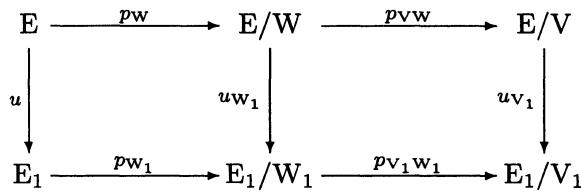
\includegraphics[keepaspectratio]{images/part002_2ec1bcbe.jpg}}

Now let \(\mu = (\mu_{\mathrm{V}})_{\mathrm{V}\in \mathcal{F}(\mathrm{E})}\) be a promeasure on \(\mathbf{E}\) . For every \(\mathrm{V}_1\in \mathcal{F}(\mathrm{E}_1)\) , set

\[
\nu_ {\mathrm{V} _ {1}} = u _ {\mathrm{V} _ {1}} \left(\mu_ {u ^ {- 1} \left(\mathrm{V} _ {1}\right)}\right).\tag{1}
\]

The commutativity of the preceding diagram shows that the family \(\nu = (\nu_{\mathrm{V}_1})_{\mathrm{V}_1 \in \mathcal{F}(\mathrm{E}_1)}\) is a promeasure on \(\mathbf{E}_1\) . We say that \(\nu\) is the image of \(\mu\) under \(u\) , and denote it by \(u(\mu)\) .

Let \(\lambda\) be a bounded measure on E, and \(u(\lambda)\) the measure on \(E_{1}\) that is the image of \(\lambda\) under u. If the promeasure \(\mu\) is associated with \(\lambda\) , then the promeasure \(u(\mu)\) is associated with \(u(\lambda)\) . This follows from the commutativity of the preceding diagram.

Let \(V \in \mathcal{F}(E)\) . It is immediate that the image promeasure on \(E/V\) of the promeasure \(\mu\) under the canonical mapping \(p_V: E \to E/V\) is associated with the measure \(\mu_V\) .

Let \(u_{1}\) be a continuous linear mapping of \(E_{1}\) into a locally convex space \(E_{2}\) . One establishes without difficulty the relation

\[
(u _ {1} \circ u) (\mu) = u _ {1} (u (\mu))
\]

(transitivity of the images of promeasures).

\subsection{Fourier transform of a promeasure}

Let E be a locally convex space and \(\mu = (\mu_{\mathrm{V}})_{\mathrm{V} \in \mathcal{F}(\mathrm{E})}\) a promeasure on E. For every continuous linear form \(x'\) on E, we denote by \(\mu_{x'}\) the measure on R that is the image under \(x'\) of the promeasure \(\mu\) on E. The Fourier transform of \(\mu\) is the function \(F\mu\) on \(E'\) defined by

\[
(\mathcal {F} \mu) (x ^ {\prime}) = \int_ {\mathbf {R}} e ^ {i t} d \mu_ {x ^ {\prime}} (t).\tag{2}
\]

Let \(\lambda\) be a bounded measure on E. The Fourier transform of \(\lambda\) is the function on \(\mathbf{E}'\) defined by

\[
(\mathcal {F} \lambda) (x ^ {\prime}) = \int_ {\mathrm{E}} e ^ {i \langle x, x ^ {\prime} \rangle} d \lambda (x).\tag{3}
\]

Let \(\mu\) be the promeasure associated with \(\lambda\) . For every \(x' \in E'\) , the measure \(\mu_{x'}\) on \(\mathbf{R}\) is the image under \(x': \mathrm{E} \to \mathbf{R}\) of the measure \(\lambda\) on \(\mathrm{E}\) ; from the formulas (2) and (3), one immediately deduces \(\mathcal{F}\mu = \mathcal{F}\lambda\) .

Let \(\mu\) be any promeasure on \(\mathbf{E}\) , and \(u\) a continuous linear mapping of \(\mathbf{E}\) into a locally convex space \(\mathbf{E}_1\) . Denote by \(^t u\) the linear mapping of \(\mathbf{E}_1'\) into \(\mathbf{E}'\) that is the transpose of \(u\) , and by \(\nu\) the promeasure \(u(\mu)\) on \(\mathbf{E}_1\) . For every \(x_1' \in \mathbf{E}_1'\) , we have \(^t u(x_1') = x_1' \circ u\) , whence

\[
\nu_ {x _ {1} ^ {\prime}} = x _ {1} ^ {\prime} (\nu) = x _ {1} ^ {\prime} (u (\mu)) = \left(x _ {1} ^ {\prime} \circ u\right) (\mu) = \mu^ {t} u \left(x _ {1} ^ {\prime}\right).
\]

Consequently,

\[
\mathscr {F} (u (\mu)) = (\mathscr {F} \mu) \circ {} ^ {t} u.\tag{4}
\]

In particular, let us take for u the canonical mapping \(p_{V}\) of E onto E/V (for \(V \in \mathcal{F}(E)\) ). The promeasure \(p_{\mathrm{V}}(\mu)\) on E/V is associated with the measure \(\mu_{V}\) , and \(^{t}p_{V}\) is an isomorphism of the dual of E/V onto the subspace \(V^{\circ}\) of \(E'\) orthogonal to V. If \((\mathrm{E}/\mathrm{V})'\) is identified with \(V^{\circ}\) by means of \(^{t}p_{V}\) , then

\[
(\mathcal {F} \mu) (x ^ {\prime}) = \int_ {\mathrm{E} / \mathrm{V}} e ^ {i \langle x, x ^ {\prime} \rangle} d \mu_ {\mathrm{V}} (x)\tag{5}
\]

for all \(x' \in V^{\circ}\) . One has \(E' = \bigcup_{V \in \mathcal{F}(E)} V^{\circ}\) , so that the preceding formula characterizes the function \(\mathcal{F}\mu\) on \(E'\) . Finally, if one sets \(x' = 0\) in (5), one sees that the total mass of \(\mu\) is equal to \((\mathcal{F}\mu)(0)\) .

PROPOSITION 3. --- Let E be a locally convex space. The mapping \(\mu \mapsto \mathcal{F}\mu\) of the set of promeasures on E into the set of functions on E' is injective.

The formula (5) permits reducing to the case that E is finite-dimensional; since every finite-dimensional space is isomorphic to a space \(R^{n}\) , we can even suppose that there exists an integer \(n \geqslant 0\) such that \(E = R^{n}\) . We therefore have to prove that if \(\mu\) is a bounded measure (not necessarily positive) on \(R^{n}\) and if

\[
\int_ {\mathbf {R} ^ {n}} e ^ {i \langle x, y \rangle} d \mu (x) = 0
\]

for every linear form \(y\) on \(\mathbf{R}^n\) , then \(\mu = 0\) .

For every integer \(m \geqslant 0\) , let \(\mathbf{G}_m\) be the subgroup \(m \cdot \mathbf{Z}^n\) of \(\mathbf{R}^n\) . Denote by \(\mathcal{C}_m\) the vector space of continuous functions \(f\) on \(\mathbf{R}^n\) such that \(f(x + a) = f(x)\) for \(x \in \mathbf{R}^n\) and \(a \in \mathbf{G}_m\) . By Prop. 8 of GT, X, §4, No.~4, every function in \(\mathcal{C}_m\) is the uniform limit of finite linear combinations of functions of the type \(x \mapsto e^{2\pi i\langle x,q\rangle}\) with \(q \in m^{-1} \cdot \mathbf{Z}^n\) . Therefore \(\mu(f) = 0\) for every function \(f \in \mathcal{C}_m\) .

Let \(f\) be a continuous function on \(\mathbf{R}^n\) with compact support. For every integer \(m \geqslant 0\) , set \(f_m(x) = \sum_{q \in G_m} f(x + q)\) . It is immediate that for every \(x \in \mathbf{R}^n\) , the preceding series has only finitely many terms, and that \(f_m\) belongs to \(\mathcal{C}_m\) . Moreover, it is easy to see that the sequence \((f_m)\) tends to \(f\) uniformly on every compact set, and that there exists a constant \(C \geqslant 0\) such that \(|f_m| \leqslant C\) for all \(m\) . Consequently, \(\mu(f) = \lim_{m \to \infty} \mu(f_m)\) by Prop. 12 of §5, No.~6. Since \(f_m \in \mathcal{C}_m\) , we have \(\mu(f_m) = 0\) , whence finally \(\mu(f) = 0\) . Thus \(\mu = 0\) .

*Remark. --- When E is finite-dimensional, every character of E is of the form \(x \mapsto e^{i\langle x,x' \rangle}\) with \(x' \in \mathrm{E}'\) (Théor. spect., Ch. II, §1, No.~9, Cor. 3 of Prop. 12). In this case, Prop. 3 follows from the uniqueness theorem for the Fourier transformation (loc. cit., §1, No.~6, Cor. of Prop. 6).*

\subsection{Calculation of Gaussian integrals}

Lemma 1. --- For every integer \(n \geqslant 0\) ,

\begin{enumerate}
\def\labelenumi{(\arabic{enumi})}
\setcounter{enumi}{5}
\tightlist
\item
\end{enumerate}

\[
\int_ {\mathbf {R}} | x | ^ {n} e ^ {- x ^ {2} / 2} d x = 2 ^ {\frac {n + 1}{2}} \Gamma \left(\frac {n + 1}{2}\right)\tag{7}
\]

\[
\int_ {\mathbf {R}} x ^ {2 n} e ^ {- x ^ {2} / 2} d x = (2 \pi) ^ {1 / 2} \frac {(2 n) !}{2 ^ {n} n !}\tag{8}
\]

\[
\int_ {\mathbf {R}} x ^ {2 n + 1} e ^ {- x ^ {2} / 2} d x = 0.
\]

Recall the formula

\[
\Gamma (s) = \int_ {0} ^ {\infty} u ^ {s - 1} e ^ {- u} d u\tag{9}
\]

valid for every real number \(s > 0\) (FRV, VII, §1, No.~3, Prop. 3). On making the change of variable \(x = (2u)^{1/2}\) , it follows from (9) that

\[
\int_ {0} ^ {\infty} x ^ {n} e ^ {- x ^ {2} / 2} d x = \int_ {0} ^ {\infty} (2 u) ^ {n / 2} e ^ {- u} \frac {1}{2} 2 ^ {1 / 2} u ^ {- 1 / 2} d u = 2 ^ {\frac {n - 1}{2}} \Gamma \left(\frac {n + 1}{2}\right),
\]

whence the formula (6) since

\[
\int_ {\mathbf {R}} | x | ^ {n} e ^ {- x ^ {2} / 2} d x = 2 \int_ {0} ^ {\infty} x ^ {n} e ^ {- x ^ {2} / 2} d x.
\]

The formula (7) follows from (6) and the relation

\[
\Gamma \left(n + \frac {1}{2}\right) = \pi^ {1 / 2} \frac {(2 n) !}{2 ^ {2 n} n !}.\tag{10}
\]

For \(n = 0\) , this relation reduces to \(\Gamma(\frac{1}{2}) = \pi^{1/2}\) , that is, to the formula (21) of FRV, VII, §1, No.~3. The general case then follows by induction on \(n\) , on taking into account the relation \(\Gamma(x + 1) = x \cdot \Gamma(x)\) (loc. cit., §1, No.~1).

Finally, the formula (8) follows from the fact that the function \(x \mapsto x^{2n+1}e^{-x^2/2}\) is odd.

Lemma 2. --- For every complex number y,

\[
(2 \pi) ^ {- 1 / 2} \int_ {\mathbf {R}} e ^ {- x ^ {2} / 2} e ^ {i x y} d x = e ^ {- y ^ {2} / 2}.\tag{11}
\]

In particular,

\[
(2 \pi) ^ {- 1 / 2} \int_ {\mathbf {R}} e ^ {- x ^ {2} / 2} d x = 1.
\]

The change of variable \(x \mapsto -x\) yields

\[
(2 \pi) ^ {- 1 / 2} \int_ {\mathbf {R}} e ^ {- x ^ {2} / 2} e ^ {i x y} d x = (2 \pi) ^ {- 1 / 2} \int_ {\mathbf {R}} e ^ {- x ^ {2} / 2} e ^ {- i x y} d x;
\]

since \(\cos u = \frac{e^{iu} + e^{-iu}}{2}\) for every complex number \(u\) , it follows that

\[
(2 \pi) ^ {- 1 / 2} \int_ {\mathbf {R}} e ^ {- x ^ {2} / 2} e ^ {i x y} d x = (2 \pi) ^ {- 1 / 2} \int_ {\mathbf {R}} e ^ {- x ^ {2} / 2} \cos x y d x.\tag{12}
\]

For every integer \(n \geqslant 0\) , set

\[
g _ {n} (x) = (- 1) ^ {n} (2 \pi) ^ {- 1 / 2} \frac {(x y) ^ {2 n}}{(2 n) !} e ^ {- x ^ {2} / 2}.
\]

By (7),

\begin{enumerate}
\def\labelenumi{(\arabic{enumi})}
\setcounter{enumi}{12}
\tightlist
\item
\end{enumerate}

\[
\int_ {\mathbf {R}} | g _ {n} (x) | d x = \frac {1}{n !} \biggl (\frac {| y | ^ {2}}{2} \biggr) ^ {n}\tag{14}
\]

\[
\int_ {\mathbf {R}} g _ {n} (x) d x = \frac {1}{n !} \Big (- \frac {y ^ {2}}{2} \Big) ^ {n},
\]

whence

\[
\sum_ {n = 0} ^ {\infty} \int_ {\mathbf {R}} | g _ {n} (x) | d x = e ^ {| y | ^ {2} / 2} <   + \infty .
\]

Since, moreover,

\[
(2 \pi) ^ {- 1 / 2} e ^ {- x ^ {2} / 2} \cos x y = \sum_ {n = 0} ^ {\infty} g _ {n} (x),
\]

this equality can be integrated term by term, whence

\[
(2 \pi) ^ {- 1 / 2} \int_ {\mathbf {R}} e ^ {- x ^ {2} / 2} \cos x y d x = \sum_ {n = 0} ^ {\infty} \int_ {\mathbf {R}} g _ {n} (x) d x = e ^ {- y ^ {2} / 2}
\]

by (14). The formula (11) then follows from (12).

\subsection{Gaussian promeasures and measures}

PROPOSITION 4. --- Let E be a locally convex space. For every positive quadratic form Q on \(E'\) , there exists one and only one promeasure \(\Gamma_{Q}\) on E such that \(F\Gamma_{Q}=e^{-Q/2}\) . The total mass of \(\Gamma_{Q}\) is equal to 1.

The uniqueness of \(\Gamma_{Q}\) follows from Prop. 3 of No.~3. The total mass of \(\Gamma_{Q}\) is equal to \((\mathcal{F}\Gamma_{\mathrm{Q}})(0)=e^{-\mathrm{Q}(0)/2}=1\) . We will prove existence in stages.

\begin{enumerate}
\def\labelenumi{\Alph{enumi})}
\tightlist
\item
  E of finite dimension n, and Q nondegenerate.
\end{enumerate}

By Lemma 2 of No.~4, the measure \(\gamma_{1}\) on R having density \(t \mapsto (2\pi)^{-1/2}e^{-t^{2}/2}\) is bounded, of total mass 1. Set \(\gamma = \gamma_{1} \otimes \cdots \otimes \gamma_{1}\) (n factors). From Lemma 2 of No.~4, one deduces

\[
\begin{array}{r l} & {\int_ {\mathbf {R} ^ {n}} e ^ {i (a _ {1} t _ {1} + \dots + a _ {n} t _ {n})} d \gamma (t _ {1}, \ldots , t _ {n}) = \prod_ {j = 1} ^ {n} \int_ {\mathbf {R}} e ^ {i a _ {j} t} d \gamma_ {1} (t)} \\ & {\qquad = \prod_ {j = 1} ^ {n} (2 \pi) ^ {- 1 / 2} \int_ {\mathbf {R}} e ^ {i a _ {j} t} e ^ {- t ^ {2} / 2} d t} \\ & {\qquad = \prod_ {j = 1} ^ {n} e ^ {- a _ {j} ^ {2} / 2}} \\ & {\qquad = \exp \big (- \frac {1}{2} (a _ {1} ^ {2} + \dots + a _ {n} ^ {2}) \big).} \end{array}
\]

Since Q is positive and nondegenerate, there exists a basis \((e_{1}^{\prime},\ldots,e_{n}^{\prime})\) of \(E^{\prime}\) orthonormal for Q (Alg., Ch. IX, §7, No.~1). Let us denote by f the isomorphism \(x\mapsto(e_{1}^{\prime}(x),\ldots,e_{n}^{\prime}(x))\) of E onto \(R^{n}\) , and by \(\Gamma_{Q}\) the measure \(f^{-1}(\gamma)\) on E. Let \(x^{\prime}=a_{1}e_{1}^{\prime}+\cdots+a_{n}e_{n}^{\prime}\) be in \(E^{\prime}\) ; then \(x^{\prime}\big(f^{-1}(t_{1},\ldots,t_{n})\big)=\sum_{j=1}^{n}t_{j}a_{j}\) for \(t_{1},\ldots,t_{n}\) real, whence

\[
\begin{array}{l} \int_ {\mathbf {E}} e ^ {i \langle x, x ^ {\prime} \rangle} d \Gamma_ {\mathbf {Q}} (x) = \int_ {\mathbf {R} ^ {n}} e ^ {i (a _ {1} t _ {1} + \dots + a _ {n} t _ {n})} d \gamma (t _ {1}, \ldots , t _ {n}) \\ \qquad = \exp \big (- \frac {1}{2} (a _ {1} ^ {2} + \dots + a _ {n} ^ {2}) = \exp \big (- \frac {1}{2} \mathbf {Q} (x ^ {\prime}) \big). \end{array}
\]

Consequently, \(\mathcal{F}\Gamma_{\mathrm{Q}} = e^{-\mathrm{Q} / 2}\) .

\begin{enumerate}
\def\labelenumi{\Alph{enumi})}
\setcounter{enumi}{1}
\tightlist
\item
  E finite-dimensional.
\end{enumerate}

Let N be the linear subspace of \(E'\) formed by the \(x'\) such that \(Q(x') = 0\) . Denote by M the orthogonal of N in E, and by j the canonical injection of M into E. The linear mapping \({}^{t}j : E' \to M'\) is surjective, with kernel N, therefore there exists on \(M'\) a nondegenerate positive quadratic form q such that \(Q = q \circ {}^{t}j\) . By the foregoing, there exists a bounded measure \(\Gamma\) on M such that \(F\Gamma = e^{-q/2}\) . Setting \(\Gamma_{Q} = j(\Gamma)\) , we have

\[
\mathcal {F} \Gamma_ {\mathrm{Q}} = (\mathcal {F} \Gamma) \circ {} ^ {t} j = \exp (- q \circ {} ^ {t} j / 2) = e ^ {- \mathrm{Q} / 2}
\]

by formula (4) of No.~3.
